\appendix
\definecolor{bg}{HTML}{D3D3D3}
\chapter{Files}

\newpage
\section{Gene YAML}\label{sec:geneYAML}

\begin{minted}
[
framesep=0mm,
baselinestretch=1.3,
bgcolor=bg,
fontsize=\footnotesize,
linenos,
breaklines
]
{yaml}
---

name: Gene
url: Gene

status: release
spec_type: Profile
group: genes
use_cases_url: /useCases/Genes/
cross_walk_url: https://docs.google.com/spreadsheets/d/15yAvj5m-Ak_hbkSGrBx2fuhTfcQh-gY1mLT1jdOu5a0/edit#gid=1483018794
gh_tasks: https://github.com/BioSchemas/bioschemas/labels/type%3A%20Gene
live_deploy: ''

parent_type: Gene
hierarchy:
- Thing
- BioChemEntity
- Gene

spec_mapping_url: https://docs.google.com/spreadsheets/d/1WGP1VPElboWsKnASQwbp19wcvTg-_piOCoIJ6Xe7rB8/edit#gid=1483018794

# spec_info content generated using GOWeb
# DO NOT MANUALLY EDIT THE CONTENT
spec_info:
  title: Gene
  subtitle: Bioschemas profile describing a Gene in Life Sciences
  description: This Gene profile specification presents the markup for describing
    a Gene.
  version: 0.4
  version_date: 20181110T092310
  official_type: http://bioschemas.org/Gene
  full_example: https://github.com/BioSchemas/Specifications/tree/master/Gene/
mapping:
- property: additionalProperty
  expected_types:
  - PropertyValue
  description: |-
    A property-value pair representing an additional characteristics of the entitity, e.g. a product feature or another characteristic for which there is no matching property in schema.org.

    Note: Publishers should be aware that applications designed to use specific schema.org properties (e.g. http://schema.org/width, http://schema.org/color, http://schema.org/gtin13, ...) will typically expect such data to be provided using those properties, rather than using the generic property/value mechanism.
  type: ""
  type_url: ""
  bsc_description: Whenever possible, please use a property coined in a third-party
    well-know vocabulary. For instance, you can directly use http://purl.obolibrary.org/obo/RO_0002327
    as a property to express how a protein or gene enables some GO molecular function.
    If you still want or need to use additionalProperty, please use (i) property name
    to specify the name of the property, (ii) additionalType (if possible) to better
    specify the nature of the property, and (iii) value to link to the object/range
    of this property.
  marginality: Optional
  cardinality: MANY
  controlled_vocab: ""
  example: ""
- property: additionalType
  expected_types:
  - URL
  description: An additional type for the item, typically used for adding more specific
    types from external vocabularies in microdata syntax. This is a relationship between
    something and a class that the thing is in. In RDFa syntax, it is better to use
    the native RDFa syntax - the 'typeof' attribute - for multiple types. Schema.org
    tools may have only weaker understanding of extra types, in particular those defined
    externally.
  type: ""
  type_url: ""
  bsc_description: |-
    Any ontology term describing the gene concept. This is in addition to the official type used in Bioschemas.

    **Bioschemas Gene**: Official proposed term for the profile describing a gene: [SO:gene](http://purl.obolibrary.org/obo/SO_0000704).
  marginality: Optional
  cardinality: MANY
  controlled_vocab: ""
  example: |-
    {
        "@type": ["Gene"],
        "additionalType": "http://semanticscience.org/resource/SIO_010035"
    }
- property: alternateName
  expected_types:
  - Text
  description: An alias for the item.
  type: ""
  type_url: ""
  bsc_description: ""
  marginality: Optional
  cardinality: MANY
  controlled_vocab: ""
  example: |-
    {
        "@type": ["Gene"],
        "alternateName": "AD1"
    }
- property: associatedDisease
  expected_types:
  - MedicalCondition
  - URL
  description: Disease associated to this BioChemEntity
  type: bioschemas
  type_url: http://bioschemas.org/associatedDisease
  bsc_description: ""
  marginality: Optional
  cardinality: ""
  controlled_vocab: ""
  example: ""
- property: description
  expected_types:
  - Text
  description: A description of the item.
  type: ""
  type_url: ""
  bsc_description: ""
  marginality: Recommended
  cardinality: ONE
  controlled_vocab: ""
  example: |-
    {
        "@type": ["Gene"],
        "description": "amyloid beta precursor"
    }
- property: enablesMF
  expected_types:
  - CategoryCode
  - PropertyValue
  description: ""
  type: external
  type_url: ' http://purl.obolibrary.org/obo/RO_0002327'
  bsc_description: "RO:0002327 (enables). GO molecular function enabled by the gene/protein.
    \nRecommended range: BioChemEntity or CategoryCode, ProteinAnnotation if evidence
    should be included."
  marginality: Optional
  cardinality: MANY
  controlled_vocab: Only the molecular function branch of [Gene Ontology (GO)](http://www.geneontology.org)
  example: |-
    //Gene enabling a GO molecular function
    {
      "@type": ["Gene"],
      "enablesMF": {
        "@type": "CategoryCode",
        "url": "http://purl.obolibrary.org/obo/GO_0000166",
        "codeValue": "GO:0000166",
        "name": "nucleotide binding"
        }
    }
- property: encodes
  expected_types:
  - BioChemEntity
  - Protein
  - URL
  description: This property is used to link to gene products encoded (even indirectly)
    from this gene such as RNA or proteins.
  type: bioschemas
  type_url: http://bioschemas.org/encodes
  bsc_description: |-
    For genes, this property is used to express in a generic way gene products encoded by this gene. Two more specific properties SIO:010082 (is translated into) and SIO:010080 (is transcribed into) should be used for (protein) translation and (RNA) transcription respectively.
    Note: bioschemas:encodes skos:closeMatch SIO:010078
  marginality: Recommended
  cardinality: MANY
  controlled_vocab: SIO
  example: "{\n  \"@type\": [\"Gene\"],\n  \"encodes\": { \n    \"@type\": [\"Protein\"],\n
    \   \"identifier\": \"uniprotkb:P05067\",\n    \"url\": \"https://www.uniprot.org/uniprot/P05067\"\n
    \ }\n}"
- property: hasBioChemEntityPart
  expected_types:
  - BioChemEntity
  description: ""
  type: bioschemas
  type_url: http://bioschemas.org/hasBioChemEntityPart
  bsc_description: |+
    For genes, it can be used to link to gene sequence annotations such as variants or so.

  marginality: Optional
  cardinality: MANY
  controlled_vocab: ""
  example: "//Contains a variant\n{\n  \"@type\": [\"Gene\"],\n  \"hasBioChemEntityPart\":
    { \n    \"@type\": \"BioChemEntity\",\n    \"additionalType\": \"http://semanticscience.org/resource/SIO_001381\",\n
    \   \"identifier\": \"rs577882423\",\n    },\n    \"url\": \"https://www.ensembl.org/Homo_sapiens/Variation/
    Summary?db=core;g=ENSG00000142192;r=21:25880550-26171128;vf=110312838\"\n
    \ }\n}\n"
- property: hasCategoryCode
  expected_types:
  - CategoryCode
  description: A Category code contained in this code set.
  type: pending
  type_url: http://pending.schema.org/hasCategoryCode
  bsc_description: ""
  marginality: Optional
  cardinality: MANY
  controlled_vocab: ""
  example: ""
- property: hasRepresentation
  expected_types:
  - PropertyValue
  - Text
  - URL
  description: A common representation such as a protein sequence or chemical structure
    for this entity. For images use schema.org/image.
  type: bioschemas
  type_url: http://bioschemas.org/hasRepresentation
  bsc_description: For genes, this property could be used, for instance, to register
    a gene sequence as its representation. If you want to better define the nature
    of the representation, use a PropertyValue as described in additionalProperty
    or a third-party ontology predicate.
  marginality: Recommended
  cardinality: MANY
  controlled_vocab: ""
  example: |-
    {
      "@type": ["Gene"],
      "hasRepresentation": "https://www.ncbi.nlm.nih.gov/
      nuccore/NC_000021.9?report=fasta&from=25880550&to=26171128&strand=true"
    }
- property: identifier
  expected_types:
  - PropertyValue
  - Text
  - URL
  description: The identifier property represents any kind of identifier for any kind
    of Thing, such as ISBNs, GTIN codes, UUIDs etc. Schema.org provides dedicated
    properties for representing many of these, either as textual strings or as URL
    (URI) links. See [background notes](http://schema.org/docs/datamodel.html#identifierBg)
    for more details.
  type: ""
  type_url: ""
  bsc_description: ""
  marginality: Minimum
  cardinality: ONE
  controlled_vocab: ""
  example: |-
    //Using a text
    {
        "@type": ["Gene"],
        "identifier": "ENSG00000142192"
    }
    //Using a URL directly (looks like a text)
    {
        "@type": ["Gene"],
        "identifier": "http://identifiers.org/ensembl:ENSG00000142192"
    }
    //Using a URL modeled as schema:URL (equivalent to the previous one but more verbose)
    {
        "@type": ["Gene"],
        "identifier": {
          "@type": "URL",
          "url": "http://identifiers.org/ensembl:ENSG00000142192"
        }
    }
- property: image
  expected_types:
  - ImageObject
  - URL
  description: An image of the item. This can be a URL or a fully described ImageObject.
  type: ""
  type_url: ""
  bsc_description: ""
  marginality: Recommended
  cardinality: ONE
  controlled_vocab: ""
  example: |
    //Using a URL directly (looks like a text)
    {
      "@type": ["Gene"],
      "image": "https://en.wikipedia.org/wiki/Amyloid_precursor_protein#/
      media/File:Ideogram_human_chromosome_21.svg"
    }
- property: involvedInBP
  expected_types:
  - CategoryCode
  - PropertyValue
  description: ""
  type: external
  type_url: ' http://purl.obolibrary.org/obo/RO_0002331'
  bsc_description: |-
    RO:0002331 (is involved in). GO biological process this gene/protein is involved in.
    Recommended range: BioChemEntity or CategoryCode, ProteinAnnotation if evidence should be included.
  marginality: Optional
  cardinality: MANY
  controlled_vocab: Only the biological process branch of [Gene Ontology (GO)](http://www.geneontology.org)
  example: |
    //Gene involved in a GO biological process
    {
      "@type": ["Gene"],
      "involvedInBP": {
        "@type": "CategoryCode",
        "url": "http://purl.obolibrary.org/obo/GO_0000278",
        "codeValue": "GO:0000278",
        "name": "mitotic cell cycle"
        }
    }
- property: isPartOfBioChemEntity
  expected_types:
  - BioChemEntity
  description: |-
    Indicates a BioChemEntity that is (in some sense) a part of this BioChemEntity.
    Inverse property: hasBioChemEntity
  type: bioschemas
  type_url: http://bioschemas.org/isPartOfBioChemEntity
  bsc_description: |-
    **Bioschemas Gene**:
    For genes, it is recommended to at least specify the DNA/chromosome containing this gene and the taxon/organism associated to it. For taxon/organism, it is a good practice to use categoryCode to point to a controlled vocabulary such as NCBI taxon or UniProt Taxonomy.
  marginality: Recommended
  cardinality: MANY
  controlled_vocab: For subcellular locations branch from GO, please use [Gene Ontology
    (GO)](http://www.geneontology.org)
  example: "//Is contained in a chromosome in positions X to Y\n{\n  \"@type\": [\"Gene\"],\n
    \ \"isPartOfBioChemEntity\": {\n    \"@type\": \"BioChemEntity\",\n    \"name\":
    \"Chromosome 21\",\n  }\n}\n//Is contained in an organism\n{\n  \"@type\": [\"Gene\"],\n
    \ \"isPartOf\": {\n    \"@type\": \"BioChemEntity\",\n    \"name\": \"Homo sapiens\",\n
    \   \"alternateName\": \"Human\",\n    \"codeCategory\": {\n      \"@type\": \"CategoryCode\",\n
    \     \"codeValue\": \"9606\",\n      \"url\": \"http://purl.bioontology.org/ontology/NCBITAXON/9606\",\n
    \     \"sameAs\": \"http://purl.uniprot.org/taxonomy/9606\",\n      \"inCodeSet\":
    {\n        \"@type\": \"CategoryCodeSet\",\n        \"name\": \"NCBI taxon\"\n
    \     } \n    }\n  }\n}"
- property: isTranscribedInto
  expected_types:
  - BioChemEntity
  description: ""
  type: external
  type_url: http://semanticscience.org/resource/SIO_010080
  bsc_description: SIO:010080 (is transcribed into). For genes, this property is used
    to link to gene products transcribed from this gene such as RNA.
  marginality: Optional
  cardinality: MANY
  controlled_vocab: SIO
  example: ""
- property: isVariantOf
  expected_types:
  - BioChemEntity
  - bioschemas:Gene
  description: ""
  type: external
  type_url: http://semanticscience.org/resource/SIO_000272
  bsc_description: 'SIO: 000272 (is variant of). Use this property to express when
    a gene is a variant of any other gene.'
  marginality: Optional
  cardinality: MANY
  controlled_vocab: SIO
  example: ""
- property: mainEntityOfPage
  expected_types:
  - CreativeWork
  - URL
  description: |-
    Indicates a page (or other CreativeWork) for which this thing is the main entity being described. See [background notes](http://schema.org/docs/datamodel.html#mainEntityBackground) for details.
    Inverse property: mainEntity.
  type: ""
  type_url: ""
  bsc_description: Link via DataRecord to the main DataRecord representing this entity
    in a dataset. It is usually preferred to use mainEntity from a DataRecord to point
    to its corresponding entity.
  marginality: Optional
  cardinality: ONE
  controlled_vocab: ""
  example: |-
    //Preferred way from DataRecord
    {

      "@type": "DataRecord",
      "@id": "http://rdf.ebi.ac.uk/resource/ensembl/ENSG00000142192"
      "mainEntity": {
        "@type": ["Gene"],
        "name": "Name and any other property for this Gene entity"
      }
    }

    //Also possible from Gene
    {
      "@type": ["Gene"],
      "mainEntityOfPage": { "@id": "http://rdf.ebi.ac.uk/resource/ensembl/ENSG00000142192" }
    }
- property: name
  expected_types:
  - Text
  description: The name of the item.
  type: ""
  type_url: ""
  bsc_description: ""
  marginality: Minimum
  cardinality: ONE
  controlled_vocab: ""
  example: |-
    {
      "@type": ["Gene"],
      "name": "APP"
    }
- property: sameAs
  expected_types:
  - URL
  description: URL of a reference Web page that unambiguously indicates the item's
    identity. E.g. the URL of the item's Wikipedia page, Wikidata entry, or official
    website.
  type: ""
  type_url: ""
  bsc_description: ""
  marginality: Optional
  cardinality: MANY
  controlled_vocab: ""
  example: |-
    {
      "@type": ["Gene"],
      "sameAs": "https://www.wikidata.org/wiki/Q14865870"
    }
- property: taxonomicRange
  expected_types:
  - Taxon
  - Text
  - URL
  description: The taxonomic grouping of the organism that expresses, encodes, or
    in someway related to the BioChemEntity.
  type: bioschemas
  type_url: taxonomicRange
  bsc_description: ""
  marginality: Optional
  cardinality: ""
  controlled_vocab: ""
  example: ""
- property: url
  expected_types:
  - URL
  description: URL of the item.
  type: ""
  type_url: ""
  bsc_description: Link to the official webpage associated to this entity.
  marginality: Recommended
  cardinality: ONE
  controlled_vocab: ""
  example: |-
    {
      "@type": ["Gene"],
      "url": "https://www.ensembl.org/Homo_sapiens/Gene/
      Summary?g=ENSG00000142192;r=21:25880550-26171128"
    }

---
\end{minted}


\newpage
\section{Gene Python Object}\label{sec:genePythonObject}
\begin{minted}
[
framesep=0mm,
baselinestretch=1.20,
bgcolor=bg,
fontsize=\footnotesize,
linenos,
breaklines
]
{json}
{
  "name": "Gene",
  "url": "Gene",
  "status": "release",
  "spec_type": "Profile",
  "group": "genes",
  "use_cases_url": "/useCases/Genes/",
  "cross_walk_url": "https://docs.google.com/spreadsheets/d/15yAvj5m-Ak_hbkSGrBx2fuhTfcQh-gY1mLT1jdOu5a0/edit#gid=1483018794",
  "gh_tasks": "https://github.com/BioSchemas/bioschemas/labels/type%3A%20Gene",
  "live_deploy": "",
  "parent_type": "Gene",
  "hierarchy": [
    "Thing",
    "BioChemEntity",
    "Gene"
  ],
  "spec_mapping_url": "https://docs.google.com/spreadsheets/d/1WGP1VPElboWsKnASQwbp19wcvTg-_piOCoIJ6Xe7rB8/edit#gid=1483018794",
  "spec_info": {
    "title": "Gene",
    "subtitle": "Bioschemas profile describing a Gene in Life Sciences",
    "description": "This Gene profile specification presents the markup for describing a Gene.",
    "version": 0.4,
    "version_date": "20181110T092310",
    "official_type": "http://bioschemas.org/Gene",
    "full_example": "https://github.com/BioSchemas/Specifications/tree/master/Gene/"
  },
  "mapping": [
    {
      "property": "additionalProperty",
      "expected_types": [
        "PropertyValue"
      ],
      "description": "A property-value pair representing an additional characteristics of the entitity, e.g. a product feature or another characteristic for which there is no matching property in schema.org.\n\nNote: Publishers should be aware that applications designed to use specific schema.org properties (e.g. http://schema.org/width, http://schema.org/color, http://schema.org/gtin13, ...) will typically expect such data to be provided using those properties, rather than using the generic property/value mechanism.",
      "type": "",
      "type_url": "",
      "bsc_description": "Whenever possible, please use a property coined in a third-party well-know vocabulary. For instance, you can directly use http://purl.obolibrary.org/obo/RO_0002327 as a property to express how a protein or gene enables some GO molecular function. If you still want or need to use additionalProperty, please use (i) property name to specify the name of the property, (ii) additionalType (if possible) to better specify the nature of the property, and (iii) value to link to the object/range of this property.",
      "marginality": "Optional",
      "cardinality": "MANY",
      "controlled_vocab": "",
      "example": ""
    },
    {
      "property": "additionalType",
      "expected_types": [
        "URL"
      ],
      "description": "An additional type for the item, typically used for adding more specific types from external vocabularies in microdata syntax. This is a relationship between something and a class that the thing is in. In RDFa syntax, it is better to use the native RDFa syntax - the 'typeof' attribute - for multiple types. Schema.org tools may have only weaker understanding of extra types, in particular those defined externally.",
      "type": "",
      "type_url": "",
      "bsc_description": "Any ontology term describing the gene concept. This is in addition to the official type used in Bioschemas.\n\n**Bioschemas Gene**: Official proposed term for the profile describing a gene: [SO:gene](http://purl.obolibrary.org/obo/SO_0000704).",
      "marginality": "Optional",
      "cardinality": "MANY",
      "controlled_vocab": "",
      "example": "{\n    \"@type\": [\"Gene\"],\n    \"additionalType\": \"http://semanticscience.org/resource/SIO_010035\"\n}"
    },
    {
      "property": "alternateName",
      "expected_types": [
        "Text"
      ],
      "description": "An alias for the item.",
      "type": "",
      "type_url": "",
      "bsc_description": "",
      "marginality": "Optional",
      "cardinality": "MANY",
      "controlled_vocab": "",
      "example": "{\n    \"@type\": [\"Gene\"],\n    \"alternateName\": \"AD1\"\n}"
    },
    {
      "property": "associatedDisease",
      "expected_types": [
        "MedicalCondition",
        "URL"
      ],
      "description": "Disease associated to this BioChemEntity",
      "type": "bioschemas",
      "type_url": "http://bioschemas.org/associatedDisease",
      "bsc_description": "",
      "marginality": "Optional",
      "cardinality": "",
      "controlled_vocab": "",
      "example": ""
    },
    {
      "property": "description",
      "expected_types": [
        "Text"
      ],
      "description": "A description of the item.",
      "type": "",
      "type_url": "",
      "bsc_description": "",
      "marginality": "Recommended",
      "cardinality": "ONE",
      "controlled_vocab": "",
      "example": "{\n    \"@type\": [\"Gene\"],\n    \"description\": \"amyloid beta precursor\"\n}"
    },
    {
      "property": "enablesMF",
      "expected_types": [
        "CategoryCode",
        "PropertyValue"
      ],
      "description": "",
      "type": "external",
      "type_url": " http://purl.obolibrary.org/obo/RO_0002327",
      "bsc_description": "RO:0002327 (enables). GO molecular function enabled by the gene/protein. \nRecommended range: BioChemEntity or CategoryCode, ProteinAnnotation if evidence should be included.",
      "marginality": "Optional",
      "cardinality": "MANY",
      "controlled_vocab": "Only the molecular function branch of [Gene Ontology (GO)](http://www.geneontology.org)",
      "example": "//Gene enabling a GO molecular function\n{\n  \"@type\": [\"Gene\"],\n  \"enablesMF\": {\n    \"@type\": \"CategoryCode\",\n    \"url\": \"http://purl.obolibrary.org/obo/GO_0000166\",\n    \"codeValue\": \"GO:0000166\",\n    \"name\": \"nucleotide binding\"\n    }\n}"
    },
    {
      "property": "encodes",
      "expected_types": [
        "BioChemEntity",
        "Protein",
        "URL"
      ],
      "description": "This property is used to link to gene products encoded (even indirectly) from this gene such as RNA or proteins.",
      "type": "bioschemas",
      "type_url": "http://bioschemas.org/encodes",
      "bsc_description": "For genes, this property is used to express in a generic way gene products encoded by this gene. Two more specific properties SIO:010082 (is translated into) and SIO:010080 (is transcribed into) should be used for (protein) translation and (RNA) transcription respectively.\nNote: bioschemas:encodes skos:closeMatch SIO:010078",
      "marginality": "Recommended",
      "cardinality": "MANY",
      "controlled_vocab": "SIO",
      "example": "{\n  \"@type\": [\"Gene\"],\n  \"encodes\": { \n    \"@type\": [\"Protein\"],\n    \"identifier\": \"uniprotkb:P05067\",\n    \"url\": \"https://www.uniprot.org/uniprot/P05067\"\n  }\n}"
    },
    {
      "property": "hasBioChemEntityPart",
      "expected_types": [
        "BioChemEntity"
      ],
      "description": "",
      "type": "bioschemas",
      "type_url": "http://bioschemas.org/hasBioChemEntityPart",
      "bsc_description": "For genes, it can be used to link to gene sequence annotations such as variants or so.\n\n",
      "marginality": "Optional",
      "cardinality": "MANY",
      "controlled_vocab": "",
      "example": "//Contains a variant\n{\n  \"@type\": [\"Gene\"],\n  \"hasBioChemEntityPart\": { \n    \"@type\": \"BioChemEntity\",\n    \"additionalType\": \"http://semanticscience.org/resource/SIO_001381\",\n    \"identifier\": \"rs577882423\",\n    },\n    \"url\": \"https://www.ensembl.org/Homo_sapiens/Variation/
      Summary?db=core;g=ENSG00000142192;r=21:25880550-26171128;vf=110312838\"\n  }\n}\n"
    },
    {
      "property": "hasCategoryCode",
      "expected_types": [
        "CategoryCode"
      ],
      "description": "A Category code contained in this code set.",
      "type": "pending",
      "type_url": "http://pending.schema.org/hasCategoryCode",
      "bsc_description": "",
      "marginality": "Optional",
      "cardinality": "MANY",
      "controlled_vocab": "",
      "example": ""
    },
    {
      "property": "hasRepresentation",
      "expected_types": [
        "PropertyValue",
        "Text",
        "URL"
      ],
      "description": "A common representation such as a protein sequence or chemical structure for this entity. For images use schema.org/image.",
      "type": "bioschemas",
      "type_url": "http://bioschemas.org/hasRepresentation",
      "bsc_description": "For genes, this property could be used, for instance, to register a gene sequence as its representation. If you want to better define the nature of the representation, use a PropertyValue as described in additionalProperty or a third-party ontology predicate.",
      "marginality": "Recommended",
      "cardinality": "MANY",
      "controlled_vocab": "",
      "example": "{\n  \"@type\": [\"Gene\"],\n  \"hasRepresentation\": \"https://www.ncbi.nlm.nih.gov/nuccore/NC_000021.9?
      report=fasta&from=25880550&to=26171128&strand=true\"\n}"
    },
    {
      "property": "identifier",
      "expected_types": [
        "PropertyValue",
        "Text",
        "URL"
      ],
      "description": "The identifier property represents any kind of identifier for any kind of Thing, such as ISBNs, GTIN codes, UUIDs etc. Schema.org provides dedicated properties for representing many of these, either as textual strings or as URL (URI) links. See [background notes](http://schema.org/docs/datamodel.html#identifierBg) for more details.",
      "type": "",
      "type_url": "",
      "bsc_description": "",
      "marginality": "Minimum",
      "cardinality": "ONE",
      "controlled_vocab": "",
      "example": "//Using a text\n{\n    \"@type\": [\"Gene\"],\n    \"identifier\": \"ENSG00000142192\"\n}\n//Using a URL directly (looks like a text)\n{\n    \"@type\": [\"Gene\"],\n    \"identifier\": \"http://identifiers.org/ensembl:ENSG00000142192\"\n}\n//Using a URL modeled as schema:URL (equivalent to the previous one but more verbose)\n{\n    \"@type\": [\"Gene\"],\n    \"identifier\": {\n      \"@type\": \"URL\",\n      \"url\": \"http://identifiers.org/ensembl:ENSG00000142192\"\n    }\n}"
    },
    {
      "property": "image",
      "expected_types": [
        "ImageObject",
        "URL"
      ],
      
      "description": "An image of the item. This can be a URL or a fully described ImageObject.",
      "type": "",
      "type_url": "",
      "bsc_description": "",
      "marginality": "Recommended",
      "cardinality": "ONE",
      "controlled_vocab": "",
      "example": "//Using a URL directly (looks like a text)\n{\n  \"@type\": [\"Gene\"],\n  \"image\": \"https://en.wikipedia.org/wiki/Amyloid_precursor_protein#/
      media/File:Ideogram_human_chromosome_21.svg\"\n}\n"
    },
    {
      "property": "involvedInBP",
      "expected_types": [
        "CategoryCode",
        "PropertyValue"
      ],
      "description": "",
      "type": "external",
      "type_url": " http://purl.obolibrary.org/obo/RO_0002331",
      "bsc_description": "RO:0002331 (is involved in). GO biological process this gene/protein is involved in.\nRecommended range: BioChemEntity or CategoryCode, ProteinAnnotation if evidence should be included.",
      "marginality": "Optional",
      "cardinality": "MANY",
      "controlled_vocab": "Only the biological process branch of [Gene Ontology (GO)](http://www.geneontology.org)",
      "example": "//Gene involved in a GO biological process\n{\n  \"@type\": [\"Gene\"],\n  \"involvedInBP\": {\n    \"@type\": \"CategoryCode\",\n    \"url\": \"http://purl.obolibrary.org/obo/GO_0000278\",\n    \"codeValue\": \"GO:0000278\",\n    \"name\": \"mitotic cell cycle\"\n    }\n}\n"
    },
    {
      "property": "isPartOfBioChemEntity",
      "expected_types": [
        "BioChemEntity"
      ],
      "description": "Indicates a BioChemEntity that is (in some sense) a part of this BioChemEntity.\nInverse property: hasBioChemEntity",
      "type": "bioschemas",
      "type_url": "http://bioschemas.org/isPartOfBioChemEntity",
      "bsc_description": "**Bioschemas Gene**:\nFor genes, it is recommended to at least specify the DNA/chromosome containing this gene and the taxon/organism associated to it. For taxon/organism, it is a good practice to use categoryCode to point to a controlled vocabulary such as NCBI taxon or UniProt Taxonomy.",
      "marginality": "Recommended",
      "cardinality": "MANY",
      "controlled_vocab": "For subcellular locations branch from GO, please use [Gene Ontology (GO)](http://www.geneontology.org)",
     
     
     
      "example": "//Is contained in a chromosome in positions X to Y\n{\n  \"@type\": [\"Gene\"],\n  \"isPartOfBioChemEntity\": {\n    \"@type\": \"BioChemEntity\",\n    \"name\": \"Chromosome 21\",\n  }\n}\n//Is contained in an organism\n{\n  \"@type\": [\"Gene\"],\n  \"isPartOf\": {\n    \"@type\": \"BioChemEntity\",\n    \"name\": \"Homo sapiens\",\n    \"alternateName\": \"Human\",\n    \"codeCategory\": {\n      \"@type\": \"CategoryCode\",\n      \"codeValue\": \"9606\",\n      \"url\": \"http://purl.bioontology.org/ontology/NCBITAXON/9606\",\n      \"sameAs\": \"http://purl.uniprot.org/taxonomy/9606\",\n      \"inCodeSet\": {\n        \"@type\": \"CategoryCodeSet\",\n        \"name\": \"NCBI taxon\"\n      } \n    }\n  }\n}"
    },
    {
      "property": "isTranscribedInto",
      "expected_types": [
        "BioChemEntity"
      ],
      "description": "",
      "type": "external",
      "type_url": "http://semanticscience.org/resource/SIO_010080",
      "bsc_description": "SIO:010080 (is transcribed into). For genes, this property is used to link to gene products transcribed from this gene such as RNA.",
      "marginality": "Optional",
      "cardinality": "MANY",
      "controlled_vocab": "SIO",
      "example": ""
    },
    {
      "property": "isVariantOf",
      "expected_types": [
        "BioChemEntity",
        "bioschemas:Gene"
      ],
      "description": "",
      "type": "external",
      "type_url": "http://semanticscience.org/resource/SIO_000272",
      "bsc_description": "SIO: 000272 (is variant of). Use this property to express when a gene is a variant of any other gene.",
      "marginality": "Optional",
      "cardinality": "MANY",
      "controlled_vocab": "SIO",
      "example": ""
    },
    {
      "property": "mainEntityOfPage",
      "expected_types": [
        "CreativeWork",
        "URL"
      ],
      "description": "Indicates a page (or other CreativeWork) for which this thing is the main entity being described. See [background notes](http://schema.org/docs/datamodel.html#mainEntityBackground) for details.\nInverse property: mainEntity.",
      "type": "",
      "type_url": "",
      "bsc_description": "Link via DataRecord to the main DataRecord representing this entity in a dataset. It is usually preferred to use mainEntity from a DataRecord to point to its corresponding entity.",
      "marginality": "Optional",
      "cardinality": "ONE",
      "controlled_vocab": "",
      "example": "//Preferred way from DataRecord\n{\n\n  \"@type\": \"DataRecord\",\n  \"@id\": \"http://rdf.ebi.ac.uk/resource/ensembl/ENSG00000142192\"\n  \"mainEntity\": {\n    \"@type\": [\"Gene\"],\n    \"name\": \"Name and any other property for this Gene entity\"\n  }\n}\n\n//Also possible from Gene\n{\n  \"@type\": [\"Gene\"],\n  \"mainEntityOfPage\": { \"@id\": \"http://rdf.ebi.ac.uk/resource/ensembl/ENSG00000142192\" }\n}"
    },
    {
      "property": "name",
      "expected_types": [
        "Text"
      ],
      "description": "The name of the item.",
      "type": "",
      "type_url": "",
      "bsc_description": "",
      "marginality": "Minimum",
      "cardinality": "ONE",
      "controlled_vocab": "",
      "example": "{\n  \"@type\": [\"Gene\"],\n  \"name\": \"APP\"\n}"
    },
    {
      "property": "sameAs",
      "expected_types": [
        "URL"
      ],
      "description": "URL of a reference Web page that unambiguously indicates the item's identity. E.g. the URL of the item's Wikipedia page, Wikidata entry, or official website.",
      "type": "",
      "type_url": "",
      "bsc_description": "",
      "marginality": "Optional",
      "cardinality": "MANY",
      "controlled_vocab": "",
      "example": "{\n  \"@type\": [\"Gene\"],\n  \"sameAs\": \"https://www.wikidata.org/wiki/Q14865870\"\n}"
    },
    {
      "property": "taxonomicRange",
      "expected_types": [
        "Taxon",
        "Text",
        "URL"
      ],
      "description": "The taxonomic grouping of the organism that expresses, encodes, or in someway related to the BioChemEntity.",
      "type": "bioschemas",
      "type_url": "taxonomicRange",
      "bsc_description": "",
      "marginality": "Optional",
      "cardinality": "",
      "controlled_vocab": "",
      "example": ""
    },
    {
      "property": "url",
      "expected_types": [
        "URL"
      ],
      "description": "URL of the item.",
      "type": "",
      "type_url": "",
      "bsc_description": "Link to the official webpage associated to this entity.",
      "marginality": "Recommended",
      "cardinality": "ONE",
      "controlled_vocab": "",
      "example": "{\n  \"@type\": [\"Gene\"],\n  \"url\": \"https://www.ensembl.org/Homo_sapiens/Gene/
      Summary?g=ENSG00000142192;r=21:25880550-26171128\"\n}"
    }
  ]
}
\end{minted}

\newpage
\section{BioChemEntity JSON-LD} \label{sec:BioChemJSONLD}
\begin{minted}
[
framesep=0mm,
baselinestretch=1.3,
bgcolor=bg,
fontsize=\footnotesize,
linenos,
breaklines
]
{json}
{
  "@context": {
    "dct": "http://purl.org/dc/terms/",
    "owl": "http://www.w3.org/2002/07/owl#",
    "rdf": "http://www.w3.org/1999/02/22-rdf-syntax-ns#",
    "rdfa": "http://www.w3.org/ns/rdfa#",
    "rdfs": "http://www.w3.org/2000/01/rdf-schema#",
    "schema": "http://schema.org/",
    "xsd": "http://www.w3.org/2001/XMLSchema#"
  },
  "@graph": [
    {
      "@id": "schema:ProteinStructure",
      "rdfs:subClassOf": {
        "@id": "schema:BioChemEntity"
      }
    },
    {
      "@id": "schema:sampleUsed",
      "schema:rangeIncludes": {
        "@id": "schema:BioChemEntity"
      }
    },
    {
      "@id": "schema:url",
      "@type": "rdf:Property",
      "rdfs:comment": "URL of the item.",
      "rdfs:label": "url",
      "schema:domainIncludes": {
        "@id": "schema:Thing"
      },
      "schema:rangeIncludes": {
        "@id": "schema:URL"
      },
      "schema:sameAs": {
        "@id": "https://schema.org/url"
      }
    },
    {
      "@id": "schema:hasHomolog",
      "schema:rangeIncludes": {
        "@id": "schema:BioChemEntity"
      }
    },
    {
      "@id": "schema:RNA",
      "rdfs:subClassOf": {
        "@id": "schema:BioChemEntity"
      }
    },
    {
      "@id": "schema:expressedIn",
      "schema:rangeIncludes": {
        "@id": "schema:BioChemEntity"
      }
    },
    {
      "@id": "schema:SequenceRange",
      "rdfs:subClassOf": {
        "@id": "schema:BioChemEntity"
      }
    },
    {
      "@id": "schema:reagent",
      "schema:rangeIncludes": {
        "@id": "schema:BioChemEntity"
      }
    },
    {
      "@id": "schema:isEncodedByBioChemEntity",
      "@type": "rdf:Property",
      "dct:source": {
        "@id": "http://www.bioschemas.org/Gene"
      },
      "rdfs:comment": "Another BioChemEntity encoding by this one. Inverse property: <a href=\"http://schema.org/encodesBioChemEntity\">encodesBioChemEntity</a>.",
      "rdfs:label": "isEncodedByBioChemEntity",
      "schema:domainIncludes": {
        "@id": "schema:BioChemEntity"
      },
      "schema:inverseOf": {
        "@id": "schema:encodesBioChemEntity"
      },
      "schema:isPartOf": {
        "@id": "http://bio.schema.org"
      },
      "schema:rangeIncludes": [
        {
          "@id": "schema:DNA"
        },
        {
          "@id": "schema:RNA"
        },
        {
          "@id": "schema:Gene"
        }
      ],
      "schema:sameAs": {
        "@id": "https://schema.org/isEncodedByBioChemEntity"
      }
    },
    {
      "@id": "schema:hasCoenzyme",
      "schema:rangeIncludes": {
        "@id": "schema:BioChemEntity"
      }
    },
    {
      "@id": "schema:disambiguatingDescription",
      "@type": "rdf:Property",
      "rdfs:comment": "A sub property of description. A short description of the item used to disambiguate from other, similar items. Information from other properties (in particular, name) may be necessary for the description to be useful for disambiguation.",
      "rdfs:label": "disambiguatingDescription",
      "rdfs:subPropertyOf": {
        "@id": "schema:description"
      },
      "schema:domainIncludes": {
        "@id": "schema:Thing"
      },
      "schema:rangeIncludes": {
        "@id": "schema:Text"
      },
      "schema:sameAs": {
        "@id": "https://schema.org/disambiguatingDescription"
      }
    },
    {
      "@id": "schema:SequenceAnnotation",
      "rdfs:subClassOf": {
        "@id": "schema:BioChemEntity"
      }
    },
    {
      "@id": "schema:Gene",
      "rdfs:subClassOf": {
        "@id": "schema:BioChemEntity"
      }
    },
    {
      "@id": "schema:associatedDisease",
      "@type": "rdf:Property",
      "dct:source": {
        "@id": "http://www.bioschemas.org/BioChemEntity"
      },
      "rdfs:comment": "Disease associated to this BioChemEntity. Such disease can be a MedicalCondition or a URL. If you want to add an evidence supporting the association, please use PropertyValue.",
      "rdfs:label": "associatedDisease",
      "schema:domainIncludes": {
        "@id": "schema:BioChemEntity"
      },
      "schema:isPartOf": {
        "@id": "http://bio.schema.org"
      },
      "schema:rangeIncludes": [
        {
          "@id": "schema:MedicalCondition"
        },
        {
          "@id": "schema:URL"
        },
        {
          "@id": "schema:PropertyValue"
        }
      ],
      "schema:sameAs": {
        "@id": "https://schema.org/associatedDisease"
      }
    },
    {
      "@id": "schema:hasOrtholog",
      "schema:rangeIncludes": {
        "@id": "schema:BioChemEntity"
      }
    },
    {
      "@id": "schema:Protein",
      "rdfs:subClassOf": {
        "@id": "schema:BioChemEntity"
      }
    },
    {
      "@id": "schema:hasBioChemEntityPart",
      "@type": "rdf:Property",
      "dct:source": {
        "@id": "http://www.bioschemas.org"
      },
      "rdfs:comment": "Indicates a BioChemEntity that (in some sense) has this BioChemEntity as a part. Inverse property: <a href=\"http://schema.org/isPartOfBioChemEntity\">isPartOfBioChemEntity</a>.",
      "rdfs:label": "hasBioChemEntityPart",
      "schema:domainIncludes": {
        "@id": "schema:BioChemEntity"
      },
      "schema:inverseOf": {
        "@id": "schema:isPartOfBioChemEntity"
      },
      "schema:isPartOf": {
        "@id": "http://bio.schema.org"
      },
      "schema:rangeIncludes": {
        "@id": "schema:BioChemEntity"
      },
      "schema:sameAs": {
        "@id": "https://schema.org/hasBioChemEntityPart"
      }
    },
    {
      "@id": "schema:boundMolecule",
      "schema:rangeIncludes": {
        "@id": "schema:BioChemEntity"
      }
    },
    {
      "@id": "schema:potentialAction",
      "@type": "rdf:Property",
      "rdfs:comment": "Indicates a potential Action, which describes an idealized action in which this thing would play an 'object' role.",
      "rdfs:label": "potentialAction",
      "schema:domainIncludes": {
        "@id": "schema:Thing"
      },
      "schema:rangeIncludes": {
        "@id": "schema:Action"
      },
      "schema:sameAs": {
        "@id": "https://schema.org/potentialAction"
      }
    },
    {
      "@id": "schema:hasSequenceAnnotation",
      "@type": "rdf:Property",
      "dct:source": {
        "@id": "http://www.bioschemas.org/BioChemEntity"
      },
      "rdfs:comment": "Pointer to a sequence annotation; please use PropertyValue if you want to include any evidence.",
      "rdfs:label": "hasSequenceAnnotation",
      "schema:domainIncludes": {
        "@id": "schema:BioChemEntity"
      },
      "schema:isPartOf": {
        "@id": "http://bio.schema.org"
      },
      "schema:rangeIncludes": [
        {
          "@id": "schema:SequneceAnnotation"
        },
        {
          "@id": "schema:PropertyValue"
        }
      ],
      "schema:sameAs": {
        "@id": "https://schema.org/hasSequenceAnnotation"
      }
    },
    {
      "@id": "schema:biologicalType",
      "schema:rangeIncludes": {
        "@id": "schema:BioChemEntity"
      }
    },
    {
      "@id": "schema:isInvolvedInBiologicalProcess",
      "@type": "rdf:Property",
      "dct:source": {
        "@id": "http://www.bioschemas.org/BioChemEntity"
      },
      "rdfs:comment": "Biological process this BioChemEntity is involved in; please use PropertyValue if you want to include any evidence.",
      "rdfs:label": "isInvolvedInBiologicalProcess",
      "schema:domainIncludes": {
        "@id": "schema:BioChemEntity"
      },
      "schema:isPartOf": {
        "@id": "http://bio.schema.org"
      },
      "schema:rangeIncludes": [
        {
          "@id": "schema:CategoryCode"
        },
        {
          "@id": "schema:PropertyValue"
        }
      ],
      "schema:sameAs": {
        "@id": "https://schema.org/isInvolvedInBiologicalProcess"
      }
    },
    {
      "@id": "schema:name",
      "@type": "rdf:Property",
      "owl:equivalentProperty": {
        "@id": "dct:title"
      },
      "rdfs:comment": "The name of the item.",
      "rdfs:label": "name",
      "rdfs:subPropertyOf": {
        "@id": "rdfs:label"
      },
      "schema:domainIncludes": {
        "@id": "schema:Thing"
      },
      "schema:rangeIncludes": {
        "@id": "schema:Text"
      },
      "schema:sameAs": {
        "@id": "https://schema.org/name"
      }
    },
    {
      "@id": "schema:ChemicalSubstance",
      "rdfs:subClassOf": {
        "@id": "schema:BioChemEntity"
      }
    },
    {
      "@id": "schema:taxonomicRange",
      "@type": "rdf:Property",
      "dct:source": {
        "@id": "http://www.bioschemas.org"
      },
      "rdfs:comment": "The taxonomic grouping of the organism that expresses, encodes, or in someway related to the BioChemEntity.",
      "rdfs:label": "taxonomicRange",
      "schema:domainIncludes": [
        {
          "@id": "schema:Phenotype"
        },
        {
          "@id": "schema:BioChemEntity"
        }
      ],
      "schema:isPartOf": {
        "@id": "http://bio.schema.org"
      },
      "schema:rangeIncludes": [
        {
          "@id": "schema:URL"
        },
        {
          "@id": "schema:CategoryCode"
        },
        {
          "@id": "schema:Taxon"
        },
        {
          "@id": "schema:Text"
        }
      ],
      "schema:sameAs": {
        "@id": "https://schema.org/taxonomicRange"
      }
    },
    {
      "@id": "schema:identifier",
      "@type": "rdf:Property",
      "owl:equivalentProperty": {
        "@id": "dct:identifier"
      },
      "rdfs:comment": "The identifier property represents any kind of identifier for any kind of <a class=\"localLink\" href=\"http://schema.org/Thing\">Thing</a>, such as ISBNs, GTIN codes, UUIDs etc. Schema.org provides dedicated properties for representing many of these, either as textual strings or as URL (URI) links.
      See <a href=\"/docs/datamodel.html#identifierBg\">background notes</a> for more details.",
      "rdfs:label": "identifier",
      "schema:domainIncludes": {
        "@id": "schema:Thing"
      },
      "schema:rangeIncludes": [
        {
          "@id": "schema:PropertyValue"
        },
        {
          "@id": "schema:URL"
        },
        {
          "@id": "schema:Text"
        }
      ],
      "schema:sameAs": {
        "@id": "https://schema.org/identifier"
      }
    },
    {
      "@id": "schema:DNA",
      "rdfs:subClassOf": {
        "@id": "schema:BioChemEntity"
      }
    },
    {
      "@id": "schema:isPartOfBioChemEntity",
      "@type": "rdf:Property",
      "dct:source": {
        "@id": "http://www.bioschemas.org"
      },
      "rdfs:comment": "Indicates a BioChemEntity that is (in some sense) a part of this BioChemEntity. Inverse property: <a href=\"http://schema.org/hasBioChemEntityPart\">hasBioChemEntityPart</a>.",
      "rdfs:label": "isPartOfBioChemEntity",
      "schema:domainIncludes": {
        "@id": "schema:BioChemEntity"
      },
      "schema:inverseOf": {
        "@id": "schema:hasBioChemEntityPart"
      },
      "schema:isPartOf": {
        "@id": "http://bio.schema.org"
      },
      "schema:rangeIncludes": {
        "@id": "schema:BioChemEntity"
      },
      "schema:sameAs": {
        "@id": "https://schema.org/isPartOfBioChemEntity"
      }
    },
    {
      "@id": "schema:bioChemSimilarity",
      "@type": "rdf:Property",
      "dct:source": {
        "@id": "http://www.bioschemas.org"
      },
      "rdfs:comment": "A similar molecular entity, e.g., obtained by fingerprint similarity algorithms.",
      "rdfs:label": "bioChemSimilarity",
      "schema:domainIncludes": {
        "@id": "schema:BioChemEntity"
      },
      "schema:isPartOf": {
        "@id": "http://bio.schema.org"
      },
      "schema:rangeIncludes": {
        "@id": "schema:BioChemEntity"
      },
      "schema:sameAs": {
        "@id": "https://schema.org/bioChemSimilarity"
      }
    },
    {
      "@id": "schema:description",
      "@type": "rdf:Property",
      "owl:equivalentProperty": {
        "@id": "dct:description"
      },
      "rdfs:comment": "A description of the item.",
      "rdfs:label": "description",
      "schema:domainIncludes": {
        "@id": "schema:Thing"
      },
      "schema:rangeIncludes": {
        "@id": "schema:Text"
      },
      "schema:sameAs": {
        "@id": "https://schema.org/description"
      }
    },
    {
      "@id": "schema:hasMolecularFunction",
      "@type": "rdf:Property",
      "dct:source": {
        "@id": "http://www.bioschemas.org/BioChemEntity"
      },
      "rdfs:comment": "Molecular function performed by this BioChemEntity; please use PropertyValue if you want to include any evidence.",
      "rdfs:label": "hasMolecularFunction",
      "schema:domainIncludes": {
        "@id": "schema:BioChemEntity"
      },
      "schema:isPartOf": {
        "@id": "http://bio.schema.org"
      },
      "schema:rangeIncludes": [
        {
          "@id": "schema:CategoryCode"
        },
        {
          "@id": "schema:PropertyValue"
        }
      ],
      "schema:sameAs": {
        "@id": "https://schema.org/hasMolecularFunction"
      }
    },
    {
      "@id": "schema:isMatchedBy",
      "@type": "rdf:Property",
      "dct:source": {
        "@id": "http://www.bioschemas.org"
      },
      "rdfs:comment": "A model matching this BioChemEntity.",
      "rdfs:label": "isMatchedBy",
      "schema:domainIncludes": {
        "@id": "schema:BioChemEntity"
      },
      "schema:isPartOf": {
        "@id": "http://bio.schema.org"
      },
      "schema:rangeIncludes": {
        "@id": "schema:SequenceMatchingModel"
      },
      "schema:sameAs": {
        "@id": "https://schema.org/isMatchedBy"
      }
    },
    {
      "@id": "schema:additionalType",
      "@type": "rdf:Property",
      "rdfs:comment": "An additional type for the item, typically used for adding more specific types from external vocabularies in microdata syntax. This is a relationship between something and a class that the thing is in. In RDFa syntax, it is better to use the native RDFa syntax - the 'typeof' attribute - for multiple types. Schema.org tools may have only weaker understanding of extra types, in particular those defined externally.",
      "rdfs:label": "additionalType",
      "rdfs:subPropertyOf": {
        "@id": "rdf:type"
      },
      "schema:domainIncludes": {
        "@id": "schema:Thing"
      },
      "schema:rangeIncludes": {
        "@id": "schema:URL"
      },
      "schema:sameAs": {
        "@id": "https://schema.org/additionalType"
      }
    },
    {
      "@id": "schema:image",
      "@type": "rdf:Property",
      "rdfs:comment": "An image of the item. This can be a <a class=\"localLink\" href=\"http://schema.org/URL\">URL</a> or a fully described <a class=\"localLink\" href=\"http://schema.org/ImageObject\">ImageObject</a>.",
      "rdfs:label": "image",
      "schema:domainIncludes": {
        "@id": "schema:Thing"
      },
      "schema:rangeIncludes": [
        {
          "@id": "schema:ImageObject"
        },
        {
          "@id": "schema:URL"
        }
      ],
      "schema:sameAs": {
        "@id": "https://schema.org/image"
      }
    },
    {
      "@id": "schema:MolecularEntity",
      "rdfs:subClassOf": {
        "@id": "schema:BioChemEntity"
      }
    },
    {
      "@id": "schema:Thing",
      "@type": "rdfs:Class",
      "rdfs:comment": "The most generic type of item.",
      "rdfs:label": "Thing",
      "schema:sameAs": {
        "@id": "https://schema.org/Thing"
      }
    },
    {
      "@id": "schema:isLocatedInSubcellularLocation",
      "@type": "rdf:Property",
      "dct:source": {
        "@id": "http://www.bioschemas.org/BioChemEntity"
      },
      
      "rdfs:comment": "Subcellular location where this BioChemEntity is located; please use PropertyValue if you want to include any evidence.",
      "rdfs:label": "isLocatedInSubcellularLocation",
      "schema:domainIncludes": {
        "@id": "schema:BioChemEntity"
      },
      "schema:isPartOf": {
        "@id": "http://bio.schema.org"
      },
      "schema:rangeIncludes": [
        {
          "@id": "schema:CategoryCode"
        },
        {
          "@id": "schema:PropertyValue"
        }
      ],
      "schema:sameAs": {
        "@id": "https://schema.org/isLocatedInSubcellularLocation"
      }
    },
    {
      "@id": "schema:Enzyme",
      "rdfs:subClassOf": {
        "@id": "schema:BioChemEntity"
      }
    },
    {
      "@id": "schema:subjectOf",
      "@type": "rdf:Property",
      "dct:source": {
        "@id": "https://github.com/schemaorg/schemaorg/issues/1670"
      },
      "rdfs:comment": "A CreativeWork or Event about this Thing..",
      "rdfs:label": "subjectOf",
      "schema:category": "issue-1670",
      "schema:domainIncludes": {
        "@id": "schema:Thing"
      },
      "schema:inverseOf": {
        "@id": "schema:about"
      },
      "schema:isPartOf": {
        "@id": "http://pending.schema.org"
      },
      "schema:rangeIncludes": [
        {
          "@id": "schema:CreativeWork"
        },
        {
          "@id": "schema:Event"
        }
      ],
      "schema:sameAs": {
        "@id": "https://schema.org/subjectOf"
      }
    },
    {
      "@id": "schema:biologicalRole",
      "@type": "rdf:Property",
      "dct:source": {
        "@id": "http://www.bioschemas.org"
      },
      "rdfs:comment": "A role played by the molecular entity within a biological context.",
      "rdfs:label": "biologicalRole",
      "schema:domainIncludes": {
        "@id": "schema:BioChemEntity"
      },
      "schema:isPartOf": {
        "@id": "http://bio.schema.org"
      },
      "schema:rangeIncludes": {
        "@id": "schema:DefinedTerm"
      },
      "schema:sameAs": {
        "@id": "https://schema.org/biologicalRole"
      }
    },
    {
      "@id": "schema:hasRepresentation",
      "@type": "rdf:Property",
      "dct:source": {
        "@id": "http://www.bioschemas.org"
      },
      "rdfs:comment": "A common representation such as a protein sequence or chemical structure for this entity. For images use schema.org/image.",
      "rdfs:label": "hasRepresentation",
      "schema:domainIncludes": {
        "@id": "schema:BioChemEntity"
      },
      "schema:isPartOf": {
        "@id": "http://bio.schema.org"
      },
      "schema:rangeIncludes": [
        {
          "@id": "schema:Text"
        },
        {
          "@id": "schema:PropertyValue"
        },
        {
          "@id": "schema:URL"
        }
      ],
      "schema:sameAs": {
        "@id": "https://schema.org/hasRepresentation"
      }
    },
    {
      "@id": "schema:encodesBioChemEntity",
      "schema:rangeIncludes": {
        "@id": "schema:BioChemEntity"
      }
    },
    {
      "@id": "schema:mainEntityOfPage",
      "@type": "rdf:Property",
      "rdfs:comment": "Indicates a page (or other CreativeWork) for which this thing is the main entity being described. See <a href=\"/docs/datamodel.html#mainEntityBackground\">background notes</a> for details.",
      "rdfs:label": "mainEntityOfPage",
      "schema:domainIncludes": {
        "@id": "schema:Thing"
      },
      "schema:inverseOf": {
        "@id": "schema:mainEntity"
      },
      "schema:rangeIncludes": [
        {
          "@id": "schema:CreativeWork"
        },
        {
          "@id": "schema:URL"
        }
      ],
      "schema:sameAs": {
        "@id": "https://schema.org/mainEntityOfPage"
      }
    },
    {
      "@id": "schema:BioChemEntity",
      "@type": "rdfs:Class",
      "dct:source": {
        "@id": "http://bioschemas.org"
      },
      "rdfs:comment": "Any biological, chemical, or biochemical thing. For example: a protein; a gene; a chemical; a synthetic chemical.",
      "rdfs:label": "BioChemEntity",
      "rdfs:subClassOf": {
        "@id": "schema:Thing"
      },
      "schema:isPartOf": {
        "@id": "http://bio.schema.org"
      },
      "schema:sameAs": {
        "@id": "https://schema.org/BioChemEntity"
      }
    },
    {
      "@id": "schema:alternateName",
      "@type": "rdf:Property",
      "rdfs:comment": "An alias for the item.",
      "rdfs:label": "alternateName",
      "schema:domainIncludes": {
        "@id": "schema:Thing"
      },
      "schema:rangeIncludes": {
        "@id": "schema:Text"
      },
      "schema:sameAs": {
        "@id": "https://schema.org/alternateName"
      }
    },
    {
      "@id": "schema:sameAs",
      "@type": "rdf:Property",
      "rdfs:comment": "URL of a reference Web page that unambiguously indicates the item's identity. E.g. the URL of the item's Wikipedia page, Wikidata entry, or official website.",
      "rdfs:label": "sameAs",
      "schema:domainIncludes": {
        "@id": "schema:Thing"
      },
      "schema:rangeIncludes": {
        "@id": "schema:URL"
      },
      "schema:sameAs": {
        "@id": "https://schema.org/sameAs"
      }
    },
    {
      "@id": "schema:bioChemInteraction",
      "@type": "rdf:Property",
      "dct:source": {
        "@id": "http://www.bioschemas.org"
      },
      "rdfs:comment": "A BioChemEntity that is known to interact with this item.",
      "rdfs:label": "bioChemInteraction",
      "schema:domainIncludes": {
        "@id": "schema:BioChemEntity"
      },
      "schema:isPartOf": {
        "@id": "http://bio.schema.org"
      },
      "schema:rangeIncludes": {
        "@id": "schema:BioChemEntity"
      },
      "schema:sameAs": {
        "@id": "https://schema.org/bioChemInteraction"
      }
    }
  ]
}
\end{minted}

\newpage
\section{Gene JSON-Schema}\label{sec:geneJSONSchema}
\begin{minted}
[
framesep=0mm,
baselinestretch=1.3,
bgcolor=bg,
fontsize=\footnotesize,
linenos,
breaklines
]
{json}
{
    "definitions": {
        "BioChemEntity": {
            "description": "Any biological, chemical, or biochemical thing. For example: a protein; a gene; a chemical; a synthetic chemical.",
            "properties": {
                "@context": {
                    "default": "http://schema.org",
                    "options": {
                        "hidden": "true"
                    },
                    "type": "string"
                },
                "@type": {
                    "default": "BioChemEntity",
                    "options": {
                        "hidden": "true"
                    },
                    "type": "string"
                },
                "additionalType": {
                    "items": {
                        "oneOf": [
                            {
                                "$ref": "#/definitions/URL",
                                "title": "URL"
                            }
                        ]
                    },
                    "title": "additionalType",
                    "type": "array"
                },
                "alternateName": {
                    "items": {
                        "oneOf": [
                            {
                                "$ref": "#/definitions/Text",
                                "title": "Text"
                            }
                        ]
                    },
                    "title": "alternateName",
                    "type": "array"
                },
                "associatedDisease": {
                    "items": {
                        "oneOf": [
                            {
                                "properties": {
                                    "@id": {
                                        "$ref": "#/definitions/URL",
                                        "title": "@id"
                                    },
                                    "@type": {
                                        "default": "BioChemEntity",
                                        "options": {
                                            "hidden": "true"
                                        },
                                        "type": "string"
                                    }
                                },
                                "required": [
                                    "@id",
                                    "@type"
                                ],
                                "title": "BioChemEntity"
                            },
                            {
                                "$ref": "#/definitions/URL",
                                "title": "URL"
                            },
                            {
                                "properties": {
                                    "@id": {
                                        "$ref": "#/definitions/URL",
                                        "title": "@id"
                                    },
                                    "@type": {
                                        "default": "BioChemEntity",
                                        "options": {
                                            "hidden": "true"
                                        },
                                        "type": "string"
                                    }
                                },
                                "required": [
                                    "@id",
                                    "@type"
                                ],
                                "title": "BioChemEntity"
                            }
                        ]
                    },
                    "title": "associatedDisease",
                    "type": "array"
                },
                "bioChemInteraction": {
                    "items": {
                        "oneOf": [
                            {
                                "properties": {
                                    "@id": {
                                        "$ref": "#/definitions/URL",
                                        "title": "@id"
                                    },
                                    "@type": {
                                        "default": "BioChemEntity",
                                        "options": {
                                            "hidden": "true"
                                        },
                                        "type": "string"
                                    }
                                },
                                "required": [
                                    "@id",
                                    "@type"
                                ],
                                "title": "BioChemEntity"
                            }
                        ]
                    },
                    "title": "bioChemInteraction",
                    "type": "array"
                },
                "bioChemSimilarity": {
                    "items": {
                        "oneOf": [
                            {
                                "properties": {
                                    "@id": {
                                        "$ref": "#/definitions/URL",
                                        "title": "@id"
                                    },
                                    "@type": {
                                        "default": "BioChemEntity",
                                        "options": {
                                            "hidden": "true"
                                        },
                                        "type": "string"
                                    }
                                },
                                "required": [
                                    "@id",
                                    "@type"
                                ],
                                "title": "BioChemEntity"
                            }
                        ]
                    },
                    "title": "bioChemSimilarity",
                    "type": "array"
                },
                "biologicalRole": {
                    "items": {
                        "oneOf": [
                            {
                                "properties": {
                                    "@id": {
                                        "$ref": "#/definitions/URL",
                                        "title": "@id"
                                    },
                                    "@type": {
                                        "default": "BioChemEntity",
                                        "options": {
                                            "hidden": "true"
                                        },
                                        "type": "string"
                                    }
                                },
                                "required": [
                                    "@id",
                                    "@type"
                                ],
                                "title": "BioChemEntity"
                            }
                        ]
                    },
                    "title": "biologicalRole",
                    "type": "array"
                },
                "description": {
                    "items": {
                        "oneOf": [
                            {
                                "$ref": "#/definitions/Text",
                                "title": "Text"
                            }
                        ]
                    },
                    "title": "description",
                    "type": "array"
                },
                "disambiguatingDescription": {
                    "items": {
                        "oneOf": [
                            {
                                "$ref": "#/definitions/Text",
                                "title": "Text"
                            }
                        ]
                    },
                    "title": "disambiguatingDescription",
                    "type": "array"
                },
                "hasBioChemEntityPart": {
                    "items": {
                        "oneOf": [
                            {
                                "properties": {
                                    "@id": {
                                        "$ref": "#/definitions/URL",
                                        "title": "@id"
                                    },
                                    "@type": {
                                        "default": "BioChemEntity",
                                        "options": {
                                            "hidden": "true"
                                        },
                                        "type": "string"
                                    }
                                },
                                "required": [
                                    "@id",
                                    "@type"
                                ],
                                "title": "BioChemEntity"
                            }
                        ]
                    },
                    "title": "hasBioChemEntityPart",
                    "type": "array"
                },
                "hasMolecularFunction": {
                    "items": {
                        "oneOf": [
                            {
                                "properties": {
                                    "@id": {
                                        "$ref": "#/definitions/URL",
                                        "title": "@id"
                                    },
                                    "@type": {
                                        "default": "BioChemEntity",
                                        "options": {
                                            "hidden": "true"
                                        },
                                        "type": "string"
                                    }
                                },
                                "required": [
                                    "@id",
                                    "@type"
                                ],
                                "title": "BioChemEntity"
                            },
                            {
                                "properties": {
                                    "@id": {
                                        "$ref": "#/definitions/URL",
                                        "title": "@id"
                                    },
                                    "@type": {
                                        "default": "BioChemEntity",
                                        "options": {
                                            "hidden": "true"
                                        },
                                        "type": "string"
                                    }
                                },
                                "required": [
                                    "@id",
                                    "@type"
                                ],
                                "title": "BioChemEntity"
                            }
                        ]
                    },
                    "title": "hasMolecularFunction",
                    "type": "array"
                },
                "hasRepresentation": {
                    "items": {
                        "oneOf": [
                            {
                                "$ref": "#/definitions/Text",
                                "title": "Text"
                            },
                            {
                                "properties": {
                                    "@id": {
                                        "$ref": "#/definitions/URL",
                                        "title": "@id"
                                    },
                                    "@type": {
                                        "default": "BioChemEntity",
                                        "options": {
                                            "hidden": "true"
                                        },
                                        "type": "string"
                                    }
                                },
                                "required": [
                                    "@id",
                                    "@type"
                                ],
                                "title": "BioChemEntity"
                            },
                            {
                                "$ref": "#/definitions/URL",
                                "title": "URL"
                            }
                        ]
                    },
                    "title": "hasRepresentation",
                    "type": "array"
                },
                "hasSequenceAnnotation": {
                    "items": {
                        "oneOf": [
                            {
                                "properties": {
                                    "@id": {
                                        "$ref": "#/definitions/URL",
                                        "title": "@id"
                                    },
                                    "@type": {
                                        "default": "BioChemEntity",
                                        "options": {
                                            "hidden": "true"
                                        },
                                        "type": "string"
                                    }
                                },
                                "required": [
                                    "@id",
                                    "@type"
                                ],
                                "title": "BioChemEntity"
                            },
                            {
                                "properties": {
                                    "@id": {
                                        "$ref": "#/definitions/URL",
                                        "title": "@id"
                                    },
                                    "@type": {
                                        "default": "BioChemEntity",
                                        "options": {
                                            "hidden": "true"
                                        },
                                        "type": "string"
                                    }
                                },
                                "required": [
                                    "@id",
                                    "@type"
                                ],
                                "title": "BioChemEntity"
                            }
                        ]
                    },
                    "title": "hasSequenceAnnotation",
                    "type": "array"
                },
                "identifier": {
                    "items": {
                        "oneOf": [
                            {
                                "properties": {
                                    "@id": {
                                        "$ref": "#/definitions/URL",
                                        "title": "@id"
                                    },
                                    "@type": {
                                        "default": "BioChemEntity",
                                        "options": {
                                            "hidden": "true"
                                        },
                                        "type": "string"
                                    }
                                },
                                "required": [
                                    "@id",
                                    "@type"
                                ],
                                "title": "BioChemEntity"
                            },
                            {
                                "$ref": "#/definitions/URL",
                                "title": "URL"
                            },
                            {
                                "$ref": "#/definitions/Text",
                                "title": "Text"
                            }
                        ]
                    },
                    "title": "identifier",
                    "type": "array"
                },
                "image": {
                    "items": {
                        "oneOf": [
                            {
                                "properties": {
                                    "@id": {
                                        "$ref": "#/definitions/URL",
                                        "title": "@id"
                                    },
                                    "@type": {
                                        "default": "BioChemEntity",
                                        "options": {
                                            "hidden": "true"
                                        },
                                        "type": "string"
                                    }
                                },
                                "required": [
                                    "@id",
                                    "@type"
                                ],
                                "title": "BioChemEntity"
                            },
                            {
                                "$ref": "#/definitions/URL",
                                "title": "URL"
                            }
                        ]
                    },
                    "title": "image",
                    "type": "array"
                },
                "isEncodedByBioChemEntity": {
                    "items": {
                        "oneOf": [
                            {
                                "properties": {
                                    "@id": {
                                        "$ref": "#/definitions/URL",
                                        "title": "@id"
                                    },
                                    "@type": {
                                        "default": "BioChemEntity",
                                        "options": {
                                            "hidden": "true"
                                        },
                                        "type": "string"
                                    }
                                },
                                "required": [
                                    "@id",
                                    "@type"
                                ],
                                "title": "BioChemEntity"
                            },
                            {
                                "properties": {
                                    "@id": {
                                        "$ref": "#/definitions/URL",
                                        "title": "@id"
                                    },
                                    "@type": {
                                        "default": "BioChemEntity",
                                        "options": {
                                            "hidden": "true"
                                        },
                                        "type": "string"
                                    }
                                },
                                "required": [
                                    "@id",
                                    "@type"
                                ],
                                "title": "BioChemEntity"
                            },
                            {
                                "properties": {
                                    "@id": {
                                        "$ref": "#/definitions/URL",
                                        "title": "@id"
                                    },
                                    "@type": {
                                        "default": "BioChemEntity",
                                        "options": {
                                            "hidden": "true"
                                        },
                                        "type": "string"
                                    }
                                },
                                "required": [
                                    "@id",
                                    "@type"
                                ],
                                "title": "BioChemEntity"
                            }
                        ]
                    },
                    "title": "isEncodedByBioChemEntity",
                    "type": "array"
                },
                "isInvolvedInBiologicalProcess": {
                    "items": {
                        "oneOf": [
                            {
                                "properties": {
                                    "@id": {
                                        "$ref": "#/definitions/URL",
                                        "title": "@id"
                                    },
                                    "@type": {
                                        "default": "BioChemEntity",
                                        "options": {
                                            "hidden": "true"
                                        },
                                        "type": "string"
                                    }
                                },
                                "required": [
                                    "@id",
                                    "@type"
                                ],
                                "title": "BioChemEntity"
                            },
                            {
                                "properties": {
                                    "@id": {
                                        "$ref": "#/definitions/URL",
                                        "title": "@id"
                                    },
                                    "@type": {
                                        "default": "BioChemEntity",
                                        "options": {
                                            "hidden": "true"
                                        },
                                        "type": "string"
                                    }
                                },
                                "required": [
                                    "@id",
                                    "@type"
                                ],
                                "title": "BioChemEntity"
                            }
                        ]
                    },
                    "title": "isInvolvedInBiologicalProcess",
                    "type": "array"
                },
                "isLocatedInSubcellularLocation": {
                    "items": {
                        "oneOf": [
                            {
                                "properties": {
                                    "@id": {
                                        "$ref": "#/definitions/URL",
                                        "title": "@id"
                                    },
                                    "@type": {
                                        "default": "BioChemEntity",
                                        "options": {
                                            "hidden": "true"
                                        },
                                        "type": "string"
                                    }
                                },
                                "required": [
                                    "@id",
                                    "@type"
                                ],
                                "title": "BioChemEntity"
                            },
                            {
                                "properties": {
                                    "@id": {
                                        "$ref": "#/definitions/URL",
                                        "title": "@id"
                                    },
                                    "@type": {
                                        "default": "BioChemEntity",
                                        "options": {
                                            "hidden": "true"
                                        },
                                        "type": "string"
                                    }
                                },
                                "required": [
                                    "@id",
                                    "@type"
                                ],
                                "title": "BioChemEntity"
                            }
                        ]
                    },
                    "title": "isLocatedInSubcellularLocation",
                    "type": "array"
                },
                "isMatchedBy": {
                    "items": {
                        "oneOf": [
                            {
                                "properties": {
                                    "@id": {
                                        "$ref": "#/definitions/URL",
                                        "title": "@id"
                                    },
                                    "@type": {
                                        "default": "BioChemEntity",
                                        "options": {
                                            "hidden": "true"
                                        },
                                        "type": "string"
                                    }
                                },
                                "required": [
                                    "@id",
                                    "@type"
                                ],
                                "title": "BioChemEntity"
                            }
                        ]
                    },
                    "title": "isMatchedBy",
                    "type": "array"
                },
                "isPartOfBioChemEntity": {
                    "items": {
                        "oneOf": [
                            {
                                "properties": {
                                    "@id": {
                                        "$ref": "#/definitions/URL",
                                        "title": "@id"
                                    },
                                    "@type": {
                                        "default": "BioChemEntity",
                                        "options": {
                                            "hidden": "true"
                                        },
                                        "type": "string"
                                    }
                                },
                                "required": [
                                    "@id",
                                    "@type"
                                ],
                                "title": "BioChemEntity"
                            }
                        ]
                    },
                    "title": "isPartOfBioChemEntity",
                    "type": "array"
                },
                "mainEntityOfPage": {
                    "items": {
                        "oneOf": [
                            {
                                "properties": {
                                    "@id": {
                                        "$ref": "#/definitions/URL",
                                        "title": "@id"
                                    },
                                    "@type": {
                                        "default": "BioChemEntity",
                                        "options": {
                                            "hidden": "true"
                                        },
                                        "type": "string"
                                    }
                                },
                                "required": [
                                    "@id",
                                    "@type"
                                ],
                                "title": "BioChemEntity"
                            },
                            {
                                "$ref": "#/definitions/URL",
                                "title": "URL"
                            }
                        ]
                    },
                    "title": "mainEntityOfPage",
                    "type": "array"
                },
                "name": {
                    "items": {
                        "oneOf": [
                            {
                                "$ref": "#/definitions/Text",
                                "title": "Text"
                            }
                        ]
                    },
                    "title": "name",
                    "type": "array"
                },
                "potentialAction": {
                    "items": {
                        "oneOf": [
                            {
                                "properties": {
                                    "@id": {
                                        "$ref": "#/definitions/URL",
                                        "title": "@id"
                                    },
                                    "@type": {
                                        "default": "BioChemEntity",
                                        "options": {
                                            "hidden": "true"
                                        },
                                        "type": "string"
                                    }
                                },
                                "required": [
                                    "@id",
                                    "@type"
                                ],
                                "title": "BioChemEntity"
                            }
                        ]
                    },
                    "title": "potentialAction",
                    "type": "array"
                },
                "sameAs": {
                    "items": {
                        "oneOf": [
                            {
                                "$ref": "#/definitions/URL",
                                "title": "URL"
                            }
                        ]
                    },
                    "title": "sameAs",
                    "type": "array"
                },
                "subjectOf": {
                    "items": {
                        "oneOf": [
                            {
                                "properties": {
                                    "@id": {
                                        "$ref": "#/definitions/URL",
                                        "title": "@id"
                                    },
                                    "@type": {
                                        "default": "BioChemEntity",
                                        "options": {
                                            "hidden": "true"
                                        },
                                        "type": "string"
                                    }
                                },
                                "required": [
                                    "@id",
                                    "@type"
                                ],
                                "title": "BioChemEntity"
                            },
                            {
                                "properties": {
                                    "@id": {
                                        "$ref": "#/definitions/URL",
                                        "title": "@id"
                                    },
                                    "@type": {
                                        "default": "BioChemEntity",
                                        "options": {
                                            "hidden": "true"
                                        },
                                        "type": "string"
                                    }
                                },
                                "required": [
                                    "@id",
                                    "@type"
                                ],
                                "title": "BioChemEntity"
                            }
                        ]
                    },
                    "title": "subjectOf",
                    "type": "array"
                },
                "taxonomicRange": {
                    "items": {
                        "oneOf": [
                            {
                                "$ref": "#/definitions/URL",
                                "title": "URL"
                            },
                            {
                                "properties": {
                                    "@id": {
                                        "$ref": "#/definitions/URL",
                                        "title": "@id"
                                    },
                                    "@type": {
                                        "default": "BioChemEntity",
                                        "options": {
                                            "hidden": "true"
                                        },
                                        "type": "string"
                                    }
                                },
                                "required": [
                                    "@id",
                                    "@type"
                                ],
                                "title": "BioChemEntity"
                            },
                            {
                                "properties": {
                                    "@id": {
                                        "$ref": "#/definitions/URL",
                                        "title": "@id"
                                    },
                                    "@type": {
                                        "default": "BioChemEntity",
                                        "options": {
                                            "hidden": "true"
                                        },
                                        "type": "string"
                                    }
                                },
                                "required": [
                                    "@id",
                                    "@type"
                                ],
                                "title": "BioChemEntity"
                            },
                            {
                                "$ref": "#/definitions/Text",
                                "title": "Text"
                            }
                        ]
                    },
                    "title": "taxonomicRange",
                    "type": "array"
                },
                "url": {
                    "items": {
                        "oneOf": [
                            {
                                "$ref": "#/definitions/URL",
                                "title": "URL"
                            }
                        ]
                    },
                    "title": "url",
                    "type": "array"
                }
            },
            "required": [
                "@type",
                "@context"
            ],
            "title": "BioChemEntity"
        },
        "Boolean": {
            "type": "boolean"
        },
        "CategoryCode": {
            "description": "A Category Code.",
            "properties": {
                "@id": {
                    "$ref": "#/definitions/URL",
                    "title": "@id"
                },
                "@type": {
                    "default": "CategoryCode",
                    "options": {
                        "hidden": "true"
                    },
                    "type": "string"
                }
            },
            "required": [
                "@id",
                "@type"
            ],
            "title": "CategoryCode"
        },
        "CreativeWork": {
            "description": "The most generic kind of creative work, including books, movies, photographs, software programs, etc.",
            "properties": {
                "@id": {
                    "$ref": "#/definitions/URL",
                    "title": "@id"
                },
                "@type": {
                    "default": "CreativeWork",
                    "options": {
                        "hidden": "true"
                    },
                    "type": "string"
                }
            },
            "required": [
                "@id",
                "@type"
            ],
            "title": "CreativeWork"
        },
        "Date": {
            "type": "string"
        },
        "DateTime": {
            "type": "string"
        },
        "Gene": {
            "description": "This Gene profile specification presents the markup for describing a Gene.",
            "properties": {
                "@context": {
                    "default": "http://schema.org",
                    "options": {
                        "hidden": "true"
                    },
                    "type": "string"
                },
                "@type": {
                    "default": "Gene",
                    "options": {
                        "hidden": "true"
                    },
                    "type": "string"
                },
                "identifier": {
                    "description": " Schema.org: The identifier property represents any kind of identifier for any kind of Thing, such as ISBNs, GTIN codes, UUIDs etc. Schema.org provides dedicated properties for representing many of these, either as textual strings or as URL (URI) links. See [background notes](http://schema.org/docs/datamodel.html#identifierBg) for more details.",
                    "oneOf": [
                        {
                            "$ref": "#/definitions/PropertyValue",
                            "title": "PropertyValue"
                        },
                        {
                            "$ref": "#/definitions/Text",
                            "title": "Text"
                        },
                        {
                            "$ref": "#/definitions/URL",
                            "title": "URL"
                        }
                    ],
                    "title": "identifier (Minimum)"
                },
                "name": {
                    "description": " Schema.org: The name of the item.",
                    "oneOf": [
                        {
                            "$ref": "#/definitions/Text",
                            "title": "Text"
                        }
                    ],
                    "title": "name (Minimum)"
                }
            },
            "required": [
                "@type",
                "@context",
                "identifier",
                "name"
            ],
            "title": "Gene",
            "type": "object"
        },
        "ImageObject": {
            "description": "An image file.",
            "properties": {
                "@id": {
                    "$ref": "#/definitions/URL",
                    "title": "@id"
                },
                "@type": {
                    "default": "ImageObject",
                    "options": {
                        "hidden": "true"
                    },
                    "type": "string"
                }
            },
            "required": [
                "@id",
                "@type"
            ],
            "title": "ImageObject"
        },
        "Integer": {
            "type": "integer"
        },
        "MedicalCondition": {
            "description": "Any condition of the human body that affects the normal functioning of a person, whether physically or mentally. Includes diseases, injuries, disabilities, disorders, syndromes, etc.",
            "properties": {
                "@id": {
                    "$ref": "#/definitions/URL",
                    "title": "@id"
                },
                "@type": {
                    "default": "MedicalCondition",
                    "options": {
                        "hidden": "true"
                    },
                    "type": "string"
                }
            },
            "required": [
                "@id",
                "@type"
            ],
            "title": "MedicalCondition"
        },
        "Number": {
            "type": "number"
        },
        "PropertyValue": {
            "description": "A property-value pair, e.g. representing a feature of a product or place. Use the 'name' property for the name of the property. If there is an additional human-readable version of the value, put that into the 'description' property.<br/><br/>\n\nAlways use specific schema.org properties when a) they exist and b) you can populate them. Using PropertyValue as a substitute will typically not trigger the same effect as using the original, specific property.",
            "properties": {
                "@id": {
                    "$ref": "#/definitions/URL",
                    "title": "@id"
                },
                "@type": {
                    "default": "PropertyValue",
                    "options": {
                        "hidden": "true"
                    },
                    "type": "string"
                }
            },
            "required": [
                "@id",
                "@type"
            ],
            "title": "PropertyValue"
        },
        "Protein": {
            "description": "This Protein profile specification presents the markup when describing a Protein.",
            "properties": {
                "@context": {
                    "default": "http://schema.org",
                    "options": {
                        "hidden": "true"
                    },
                    "type": "string"
                },
                "@type": {
                    "default": "Protein",
                    "options": {
                        "hidden": "true"
                    },
                    "type": "string"
                },
                "identifier": {
                    "description": " Schema.org: The identifier property represents any kind of identifier for any kind of Thing, such as ISBNs, GTIN codes, UUIDs etc. Schema.org provides dedicated properties for representing many of these, either as textual strings or as URL (URI) links. See [background notes](http://schema.org/docs/datamodel.html#identifierBg) for more details.",
                    "oneOf": [
                        {
                            "$ref": "#/definitions/PropertyValue",
                            "title": "PropertyValue"
                        },
                        {
                            "$ref": "#/definitions/Text",
                            "title": "Text"
                        },
                        {
                            "$ref": "#/definitions/URL",
                            "title": "URL"
                        }
                    ],
                    "title": "identifier (Minimum)"
                },
                "name": {
                    "description": " Schema.org: The name of the item.",
                    "oneOf": [
                        {
                            "$ref": "#/definitions/Text",
                            "title": "Text"
                        }
                    ],
                    "title": "name (Minimum)"
                }
            },
            "required": [
                "@type",
                "@context",
                "identifier",
                "name"
            ],
            "title": "Protein",
            "type": "object"
        },
        "String": {
            "type": "string"
        },
        "Taxon": {
            "description": "This profile aims to denote a taxon by common properties such as its scientific name, authority, taxonomic rank and vernacular names. It is also a means to link to existing taxonomic registers where each taxon has a URI.",
            "properties": {
                "@context": {
                    "default": "http://schema.org",
                    "options": {
                        "hidden": "true"
                    },
                    "type": "string"
                },
                "@type": {
                    "default": "Taxon",
                    "options": {
                        "hidden": "true"
                    },
                    "type": "string"
                },
                "name": {
                    "description": " Bioschemas.org: Taxon name without authorship nor date information of the currently valid (zoological) or accepted (botanical) taxon. Schema.org: The name of the item.",
                    "oneOf": [
                        {
                            "$ref": "#/definitions/Text",
                            "title": "Text"
                        }
                    ],
                    "title": "name (Minimum)"
                }
            },
            "required": [
                "@type",
                "@context",
                "name"
            ],
            "title": "Taxon",
            "type": "object"
        },
        "Text": {
            "format": "text",
            "type": "string"
        },
        "URL": {
            "format": "url",
            "type": "string"
        }
    },
    "description": "This Gene profile specification presents the markup for describing a Gene.",
    "properties": {
        "@context": {
            "default": "http://schema.org",
            "options": {
                "hidden": "true"
            },
            "type": "string"
        },
        "@type": {
            "default": "Gene",
            "options": {
                "hidden": "true"
            },
            "type": "string"
        },
        "additionalProperty": {
            "description": " Bioschemas.org: Whenever possible, please use a property coined in a third-party well-know vocabulary. For instance, you can directly use http://purl.obolibrary.org/obo/RO_0002327 as a property to express how a protein or gene enables some GO molecular function. If you still want or need to use additionalProperty, please use (i) property name to specify the name of the property, (ii) additionalType (if possible) to better specify the nature of the property, and (iii) value to link to the object/range of this property. Schema.org: A property-value pair representing an additional characteristics of the entitity, e.g. a product feature or another characteristic for which there is no matching property in schema.org.\n\nNote: Publishers should be aware that applications designed to use specific schema.org properties (e.g. http://schema.org/width, http://schema.org/color, http://schema.org/gtin13, ...) will typically expect such data to be provided using those properties, rather than using the generic property/value mechanism.",
            "items": {
                "oneOf": [
                    {
                        "$ref": "#/definitions/PropertyValue",
                        "title": "PropertyValue"
                    }
                ]
            },
            "propertyOrder": 3,
            "title": "additionalProperty (Optional)",
            "type": "array"
        },
        
        
        
        "additionalType": {
            "description": " Bioschemas.org: Any ontology term describing the gene concept. This is in addition to the official type used in Bioschemas.\n\n**Bioschemas Gene**: Official proposed term for the profile describing a gene: [SO:gene](http://purl.obolibrary.org/obo/SO_0000704). Schema.org: An additional type for the item, typically used for adding more specific types from external vocabularies in microdata syntax. This is a relationship between something and a class that the thing is in. In RDFa syntax, it is better to use the native RDFa syntax - the 'typeof' attribute - for multiple types. Schema.org tools may have only weaker understanding of extra types, in particular those defined externally.",
            "items": {
                "oneOf": [
                    {
                        "$ref": "#/definitions/URL",
                        "title": "URL"
                    }
                ]
            },
            "propertyOrder": 3,
            "title": "additionalType (Optional)",
            "type": "array"
        },
        "alternateName": {
            "description": " Schema.org: An alias for the item.",
            "items": {
                "oneOf": [
                    {
                        "$ref": "#/definitions/Text",
                        "title": "Text"
                    }
                ]
            },
            "propertyOrder": 3,
            "title": "alternateName (Optional)",
            "type": "array"
        },
        "associatedDisease": {
            "description": " Schema.org: Disease associated to this BioChemEntity",
            "propertyOrder": 3,
            "title": "associatedDisease (Optional)"
        },
        "description": {
            "description": " Schema.org: A description of the item.",
            "oneOf": [
                {
                    "$ref": "#/definitions/Text",
                    "title": "Text"
                }
            ],
            "propertyOrder": 2,
            "title": "description (Recommended)"
        },
        "enablesMF": {
            "description": " Bioschemas.org: RO:0002327 (enables). GO molecular function enabled by the gene/protein. \nRecommended range: BioChemEntity or CategoryCode, ProteinAnnotation if evidence should be included.",
            "items": {
                "oneOf": [
                    {
                        "$ref": "#/definitions/CategoryCode",
                        "title": "CategoryCode"
                    },
                    {
                        "$ref": "#/definitions/PropertyValue",
                        "title": "PropertyValue"
                    }
                ]
            },
            "propertyOrder": 3,
            "title": "enablesMF (Optional)",
            "type": "array"
        },
        "encodes": {
            "description": " Bioschemas.org: For genes, this property is used to express in a generic way gene products encoded by this gene. Two more specific properties SIO:010082 (is translated into) and SIO:010080 (is transcribed into) should be used for (protein) translation and (RNA) transcription respectively.\nNote: bioschemas:encodes skos:closeMatch SIO:010078 Schema.org: This property is used to link to gene products encoded (even indirectly) from this gene such as RNA or proteins.",
            "items": {
                "oneOf": [
                    {
                        "$ref": "#/definitions/BioChemEntity",
                        "title": "BioChemEntity"
                    },
                    {
                        "$ref": "#/definitions/Protein",
                        "title": "Protein"
                    },
                    {
                        "$ref": "#/definitions/URL",
                        "title": "URL"
                    }
                ]
            },
            "propertyOrder": 2,
            "title": "encodes (Recommended)",
            "type": "array"
        },
        "hasBioChemEntityPart": {
            "description": " Bioschemas.org: For genes, it can be used to link to gene sequence annotations such as variants or so.\n\n",
            "items": {
                "oneOf": [
                    {
                        "$ref": "#/definitions/BioChemEntity",
                        "title": "BioChemEntity"
                    }
                ]
            },
            "propertyOrder": 3,
            "title": "hasBioChemEntityPart (Optional)",
            "type": "array"
        },
        "hasCategoryCode": {
            "description": " Schema.org: A Category code contained in this code set.",
            "items": {
                "oneOf": [
                    {
                        "$ref": "#/definitions/CategoryCode",
                        "title": "CategoryCode"
                    }
                ]
            },
            "propertyOrder": 3,
            "title": "hasCategoryCode (Optional)",
            "type": "array"
        },
        "hasRepresentation": {
            "description": " Bioschemas.org: For genes, this property could be used, for instance, to register a gene sequence as its representation. If you want to better define the nature of the representation, use a PropertyValue as described in additionalProperty or a third-party ontology predicate. Schema.org: A common representation such as a protein sequence or chemical structure for this entity. For images use schema.org/image.",
            "items": {
                "oneOf": [
                    {
                        "$ref": "#/definitions/PropertyValue",
                        "title": "PropertyValue"
                    },
                    {
                        "$ref": "#/definitions/Text",
                        "title": "Text"
                    },
                    {
                        "$ref": "#/definitions/URL",
                        "title": "URL"
                    }
                ]
            },
            "propertyOrder": 2,
            "title": "hasRepresentation (Recommended)",
            "type": "array"
        },
        
        
        "identifier": {
            "description": " Schema.org: The identifier property represents any kind of identifier for any kind of Thing, such as ISBNs, GTIN codes, UUIDs etc. Schema.org provides dedicated properties for representing many of these, either as textual strings or as URL (URI) links. See [background notes](http://schema.org/docs/datamodel.html#identifierBg) for more details.",
            "oneOf": [
                {
                    "$ref": "#/definitions/PropertyValue",
                    "title": "PropertyValue"
                },
                {
                    "$ref": "#/definitions/Text",
                    "title": "Text"
                },
                {
                    "$ref": "#/definitions/URL",
                    "title": "URL"
                }
            ],
            "propertyOrder": 1,
            "title": "identifier (Minimum)"
        },
        "image": {
            "description": " Schema.org: An image of the item. This can be a URL or a fully described ImageObject.",
            "oneOf": [
                {
                    "$ref": "#/definitions/ImageObject",
                    "title": "ImageObject"
                },
                {
                    "$ref": "#/definitions/URL",
                    "title": "URL"
                }
            ],
            "propertyOrder": 2,
            "title": "image (Recommended)"
        },
        "involvedInBP": {
            "description": " Bioschemas.org: RO:0002331 (is involved in). GO biological process this gene/protein is involved in.\nRecommended range: BioChemEntity or CategoryCode, ProteinAnnotation if evidence should be included.",
            "items": {
                "oneOf": [
                    {
                        "$ref": "#/definitions/CategoryCode",
                        "title": "CategoryCode"
                    },
                    {
                        "$ref": "#/definitions/PropertyValue",
                        "title": "PropertyValue"
                    }
                ]
            },
            "propertyOrder": 3,
            "title": "involvedInBP (Optional)",
            "type": "array"
        },
        "isPartOfBioChemEntity": {
            "description": " Bioschemas.org: **Bioschemas Gene**:\nFor genes, it is recommended to at least specify the DNA/chromosome containing this gene and the taxon/organism associated to it. For taxon/organism, it is a good practice to use categoryCode to point to a controlled vocabulary such as NCBI taxon or UniProt Taxonomy. Schema.org: Indicates a BioChemEntity that is (in some sense) a part of this BioChemEntity.\nInverse property: hasBioChemEntity",
            "items": {
                "oneOf": [
                    {
                        "$ref": "#/definitions/BioChemEntity",
                        "title": "BioChemEntity"
                    }
                ]
            },
            "propertyOrder": 2,
            "title": "isPartOfBioChemEntity (Recommended)",
            "type": "array"
        },
        "isTranscribedInto": {
            "description": " Bioschemas.org: SIO:010080 (is transcribed into). For genes, this property is used to link to gene products transcribed from this gene such as RNA.",
            "items": {
                "oneOf": [
                    {
                        "$ref": "#/definitions/BioChemEntity",
                        "title": "BioChemEntity"
                    }
                ]
            },
            "propertyOrder": 3,
            "title": "isTranscribedInto (Optional)",
            "type": "array"
        },
        "isVariantOf": {
            "description": " Bioschemas.org: SIO: 000272 (is variant of). Use this property to express when a gene is a variant of any other gene.",
            "items": {
                "oneOf": [
                    {
                        "$ref": "#/definitions/BioChemEntity",
                        "title": "BioChemEntity"
                    },
                    {
                        "$ref": "#/definitions/Gene",
                        "title": "Gene"
                    }
                ]
            },
            "propertyOrder": 3,
            "title": "isVariantOf (Optional)",
            "type": "array"
        },
        "mainEntityOfPage": {
            "description": " Bioschemas.org: Link via DataRecord to the main DataRecord representing this entity in a dataset. It is usually preferred to use mainEntity from a DataRecord to point to its corresponding entity. Schema.org: Indicates a page (or other CreativeWork) for which this thing is the main entity being described. See [background notes](http://schema.org/docs/datamodel.html#mainEntityBackground) for details.\nInverse property: mainEntity.",
            "oneOf": [
                {
                    "$ref": "#/definitions/CreativeWork",
                    "title": "CreativeWork"
                },
                {
                    "$ref": "#/definitions/URL",
                    "title": "URL"
                }
            ],
            "propertyOrder": 3,
            "title": "mainEntityOfPage (Optional)"
        },
        "name": {
            "description": " Schema.org: The name of the item.",
            "oneOf": [
                {
                    "$ref": "#/definitions/Text",
                    "title": "Text"
                }
            ],
            "propertyOrder": 1,
            "title": "name (Minimum)"
        },
        "sameAs": {
            "description": " Schema.org: URL of a reference Web page that unambiguously indicates the item's identity. E.g. the URL of the item's Wikipedia page, Wikidata entry, or official website.",
            "items": {
                "oneOf": [
                    {
                        "$ref": "#/definitions/URL",
                        "title": "URL"
                    }
                ]
            },
            "propertyOrder": 3,
            "title": "sameAs (Optional)",
            "type": "array"
        },
        "taxonomicRange": {
            "description": " Schema.org: The taxonomic grouping of the organism that expresses, encodes, or in someway related to the BioChemEntity.",
            "propertyOrder": 3,
            "title": "taxonomicRange (Optional)"
        },
        "url": {
            "description": " Bioschemas.org: Link to the official webpage associated to this entity. Schema.org: URL of the item.",
            "oneOf": [
                {
                    "$ref": "#/definitions/URL",
                    "title": "URL"
                }
            ],
            "propertyOrder": 2,
            "title": "url (Recommended)"
        }
    },
    "required": [
        "@type",
        "@context",
        "identifier",
        "name"
    ],
    "title": "Gene (v0.4)",
    "type": "object"
}
\end{minted}

\newpage
\section{Gene Additional Information JSON}\label{sec:geneAdditionalInformation}
\begin{minted}
[
framesep=0mm,
baselinestretch=1.3,
bgcolor=bg,
fontsize=\footnotesize,
linenos,
breaklines
]
{json}
{
    "additionalType": {
        "example": "{\n    \"@type\": [\"Gene\"],\n    \"additionalType\": \"http://semanticscience.org/resource/SIO_010035\"\n}",
        "marginality": "Optional"
    },
    "alternateName": {
        "example": "{\n    \"@type\": [\"Gene\"],\n    \"alternateName\": \"AD1\"\n}",
        "marginality": "Optional"
    },
    "description": {
        "example": "{\n    \"@type\": [\"Gene\"],\n    \"description\": \"amyloid beta precursor\"\n}",
        "marginality": "Recommended"
    },
    "enablesMF": {
        "controlled_vocab": "Only the molecular function branch of [Gene Ontology (GO)](http://www.geneontology.org)",
        "example": "//Gene enabling a GO molecular function\n{\n  \"@type\": [\"Gene\"],\n  \"enablesMF\": {\n    \"@type\": \"CategoryCode\",\n    \"url\": \"http://purl.obolibrary.org/obo/GO_0000166\",\n    \"codeValue\": \"GO:0000166\",\n    \"name\": \"nucleotide binding\"\n    }\n}",
        "marginality": "Optional"
    },
    "encodes": {
        "controlled_vocab": "SIO",
        "example": "{\n  \"@type\": [\"Gene\"],\n  \"encodes\": { \n    \"@type\": [\"Protein\"],\n    \"identifier\": \"uniprotkb:P05067\",\n    \"url\": \"https://www.uniprot.org/uniprot/P05067\"\n  }\n}",
        "marginality": "Recommended"
    },
    "hasBioChemEntityPart": {
        "example": "//Contains a variant\n{\n  \"@type\": [\"Gene\"],\n  \"hasBioChemEntityPart\": { \n    \"@type\": \"BioChemEntity\",\n    \"additionalType\": \"http://semanticscience.org/resource/SIO_001381\",\n    \"identifier\": \"rs577882423\",\n    },\n    \"url\": \"https://www.ensembl.org/Homo_sapiens/Variation/
        Summary?db=core;g=ENSG00000142192;r=21:25880550-26171128;vf=110312838\"\n  }\n}\n",
        "marginality": "Optional"
    },
    "hasRepresentation": {
        "example": "{\n  \"@type\": [\"Gene\"],\n  \"hasRepresentation\": \"https://www.ncbi.nlm.nih.gov/nuccore/
        NC_000021.9?report=fasta&from=25880550&to=26171128&strand=true\"\n}",
        "marginality": "Recommended"
    },
    
    
    "identifier": {
        "example": "//Using a text\n{\n    \"@type\": [\"Gene\"],\n    \"identifier\": \"ENSG00000142192\"\n}\n//Using a URL directly (looks like a text)\n{\n    \"@type\": [\"Gene\"],\n    \"identifier\": \"http://identifiers.org/ensembl:ENSG00000142192\"\n}\n//Using a URL modeled as schema:URL (equivalent to the previous one but more verbose)\n{\n    \"@type\": [\"Gene\"],\n    \"identifier\": {\n      \"@type\": \"URL\",\n      \"url\": \"http://identifiers.org/ensembl:ENSG00000142192\"\n    }\n}",
        "marginality": "Minimum"
    },
    "image": {
        "example": "//Using a URL directly (looks like a text)\n{\n  \"@type\": [\"Gene\"],\n  \"image\": \"https://en.wikipedia.org/wiki/Amyloid_precursor_protein#
        /media/File:Ideogram_human_chromosome_21.svg\"\n}\n",
        "marginality": "Recommended"
    },
    "involvedInBP": {
        "controlled_vocab": "Only the biological process branch of [Gene Ontology (GO)](http://www.geneontology.org)",
        "example": "//Gene involved in a GO biological process\n{\n  \"@type\": [\"Gene\"],\n  \"involvedInBP\": {\n    \"@type\": \"CategoryCode\",\n    \"url\": \"http://purl.obolibrary.org/obo/GO_0000278\",\n    \"codeValue\": \"GO:0000278\",\n    \"name\": \"mitotic cell cycle\"\n    }\n}\n",
        "marginality": "Optional"
    },
    "isPartOfBioChemEntity": {
        "controlled_vocab": "For subcellular locations branch from GO, please use [Gene Ontology (GO)](http://www.geneontology.org)",
        "example": "//Is contained in a chromosome in positions X to Y\n{\n  \"@type\": [\"Gene\"],\n  \"isPartOfBioChemEntity\": {\n    \"@type\": \"BioChemEntity\",\n    \"name\": \"Chromosome 21\",\n  }\n}\n//Is contained in an organism\n{\n  \"@type\": [\"Gene\"],\n  \"isPartOf\": {\n    \"@type\": \"BioChemEntity\",\n    \"name\": \"Homo sapiens\",\n    \"alternateName\": \"Human\",\n    \"codeCategory\": {\n      \"@type\": \"CategoryCode\",\n      \"codeValue\": \"9606\",\n      \"url\": \"http://purl.bioontology.org/ontology/NCBITAXON/9606\",\n      \"sameAs\": \"http://purl.uniprot.org/taxonomy/9606\",\n      \"inCodeSet\": {\n        \"@type\": \"CategoryCodeSet\",\n        \"name\": \"NCBI taxon\"\n      } \n    }\n  }\n}",
        "marginality": "Recommended"
    },
    "isTranscribedInto": {
        "controlled_vocab": "SIO",
        "marginality": "Optional"
    },
    "isVariantOf": {
        "controlled_vocab": "SIO",
        "marginality": "Optional"
    },
    
    
    
    "mainEntityOfPage": {
        "example": "//Preferred way from DataRecord\n{\n\n  \"@type\": \"DataRecord\",\n  \"@id\": \"http://rdf.ebi.ac.uk/resource/ensembl/ENSG00000142192\"\n  \"mainEntity\": {\n    \"@type\": [\"Gene\"],\n    \"name\": \"Name and any other property for this Gene entity\"\n  }\n}\n\n//Also possible from Gene\n{\n  \"@type\": [\"Gene\"],\n  \"mainEntityOfPage\": { \"@id\": \"http://rdf.ebi.ac.uk/resource/ensembl/ENSG00000142192\" }\n}",
        "marginality": "Optional"
    },
    "name": {
        "example": "{\n  \"@type\": [\"Gene\"],\n  \"name\": \"APP\"\n}",
        "marginality": "Minimum"
    },
    "sameAs": {
        "example": "{\n  \"@type\": [\"Gene\"],\n  \"sameAs\": \"https://www.wikidata.org/wiki/Q14865870\"\n}",
        "marginality": "Optional"
    },
    "url": {
        "example": "{\n  \"@type\": [\"Gene\"],\n  \"url\": \"https://www.ensembl.org/Homo_sapiens
        /Gene/Summary?g=ENSG00000142192;r=21:25880550-26171128\"\n}",
        "marginality": "Recommended"
    }
}
\end{minted}

\chapter{Prototype Usability Study} 

\newpage
\section{Questionnaire}\label{chp:prototypeUsabilityQuestionaire}
\vspace*{3.7em}
\begin{centering}
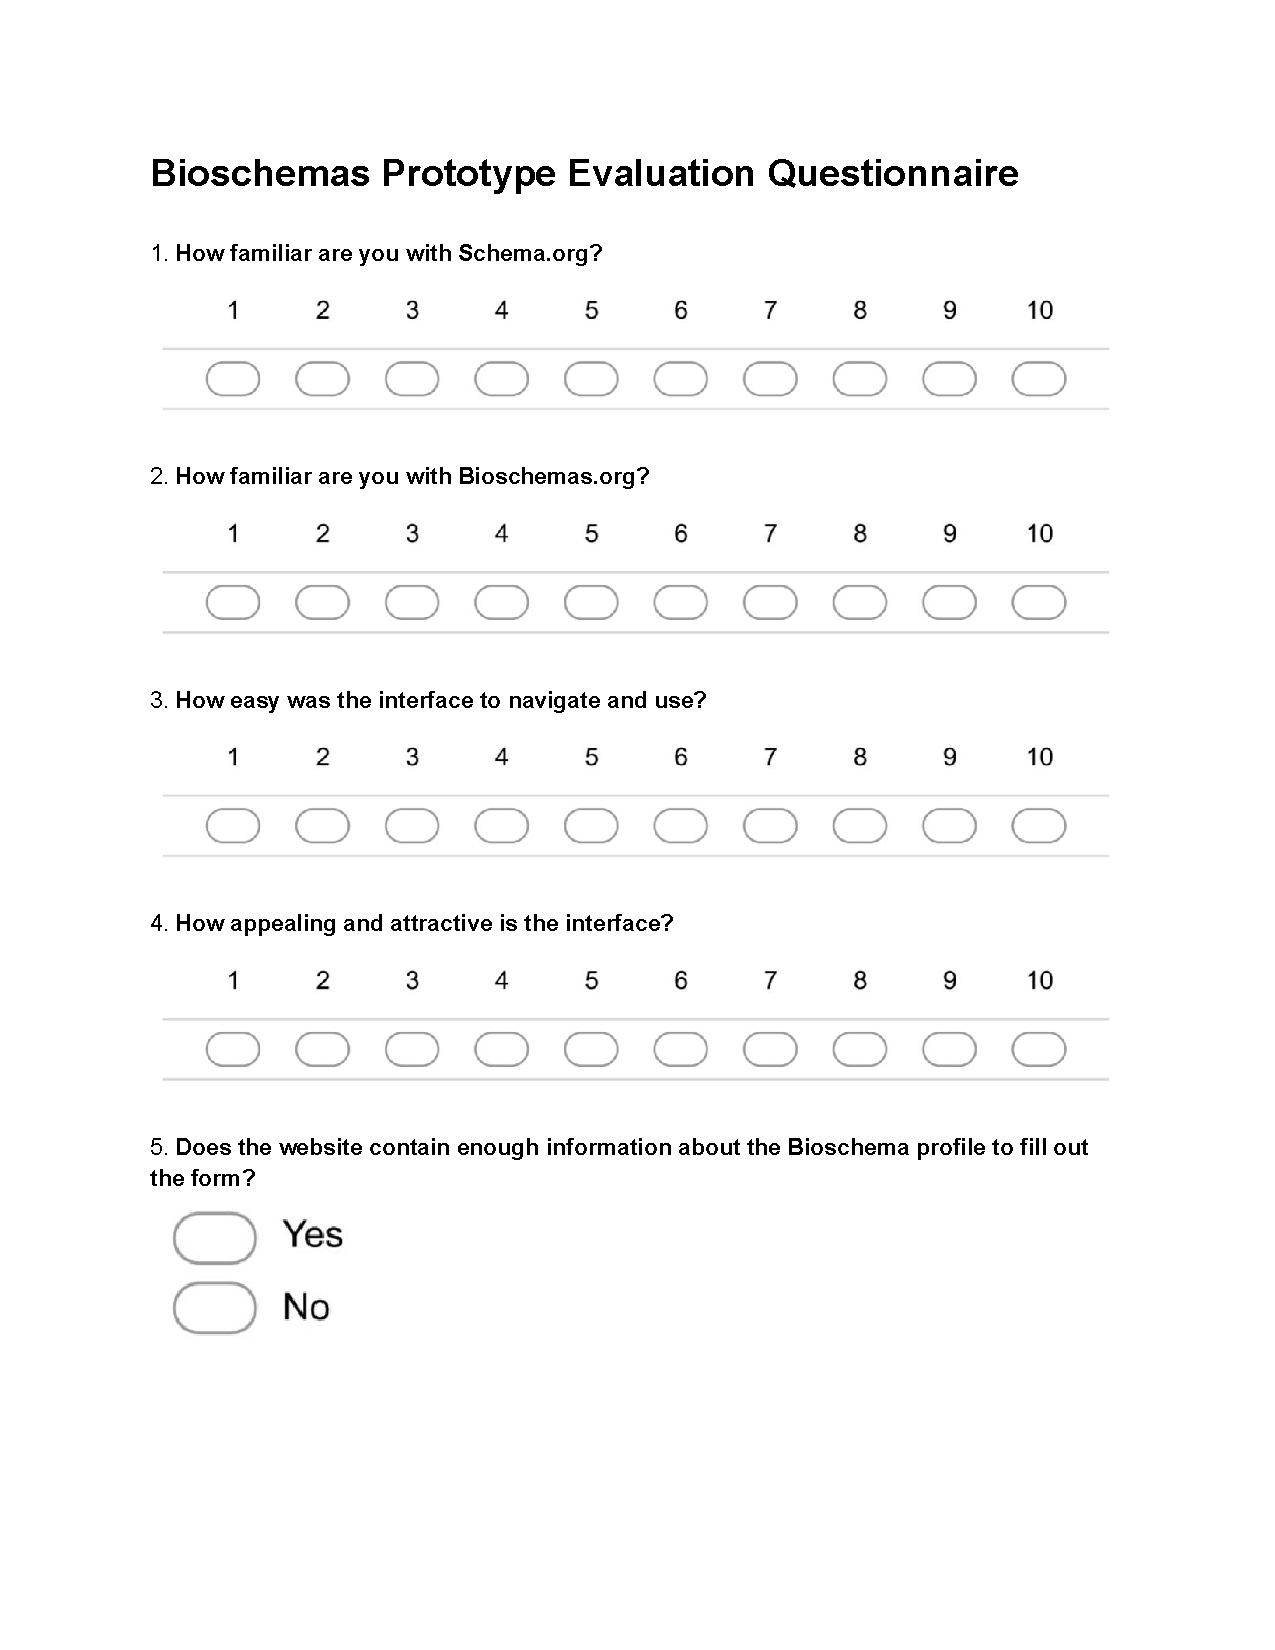
\includegraphics[trim = 40 160 0 60,scale=0.9]{forms/prototypeEvaluationFormPage1.pdf}
\end{centering}

\newpage
\begin{centering}
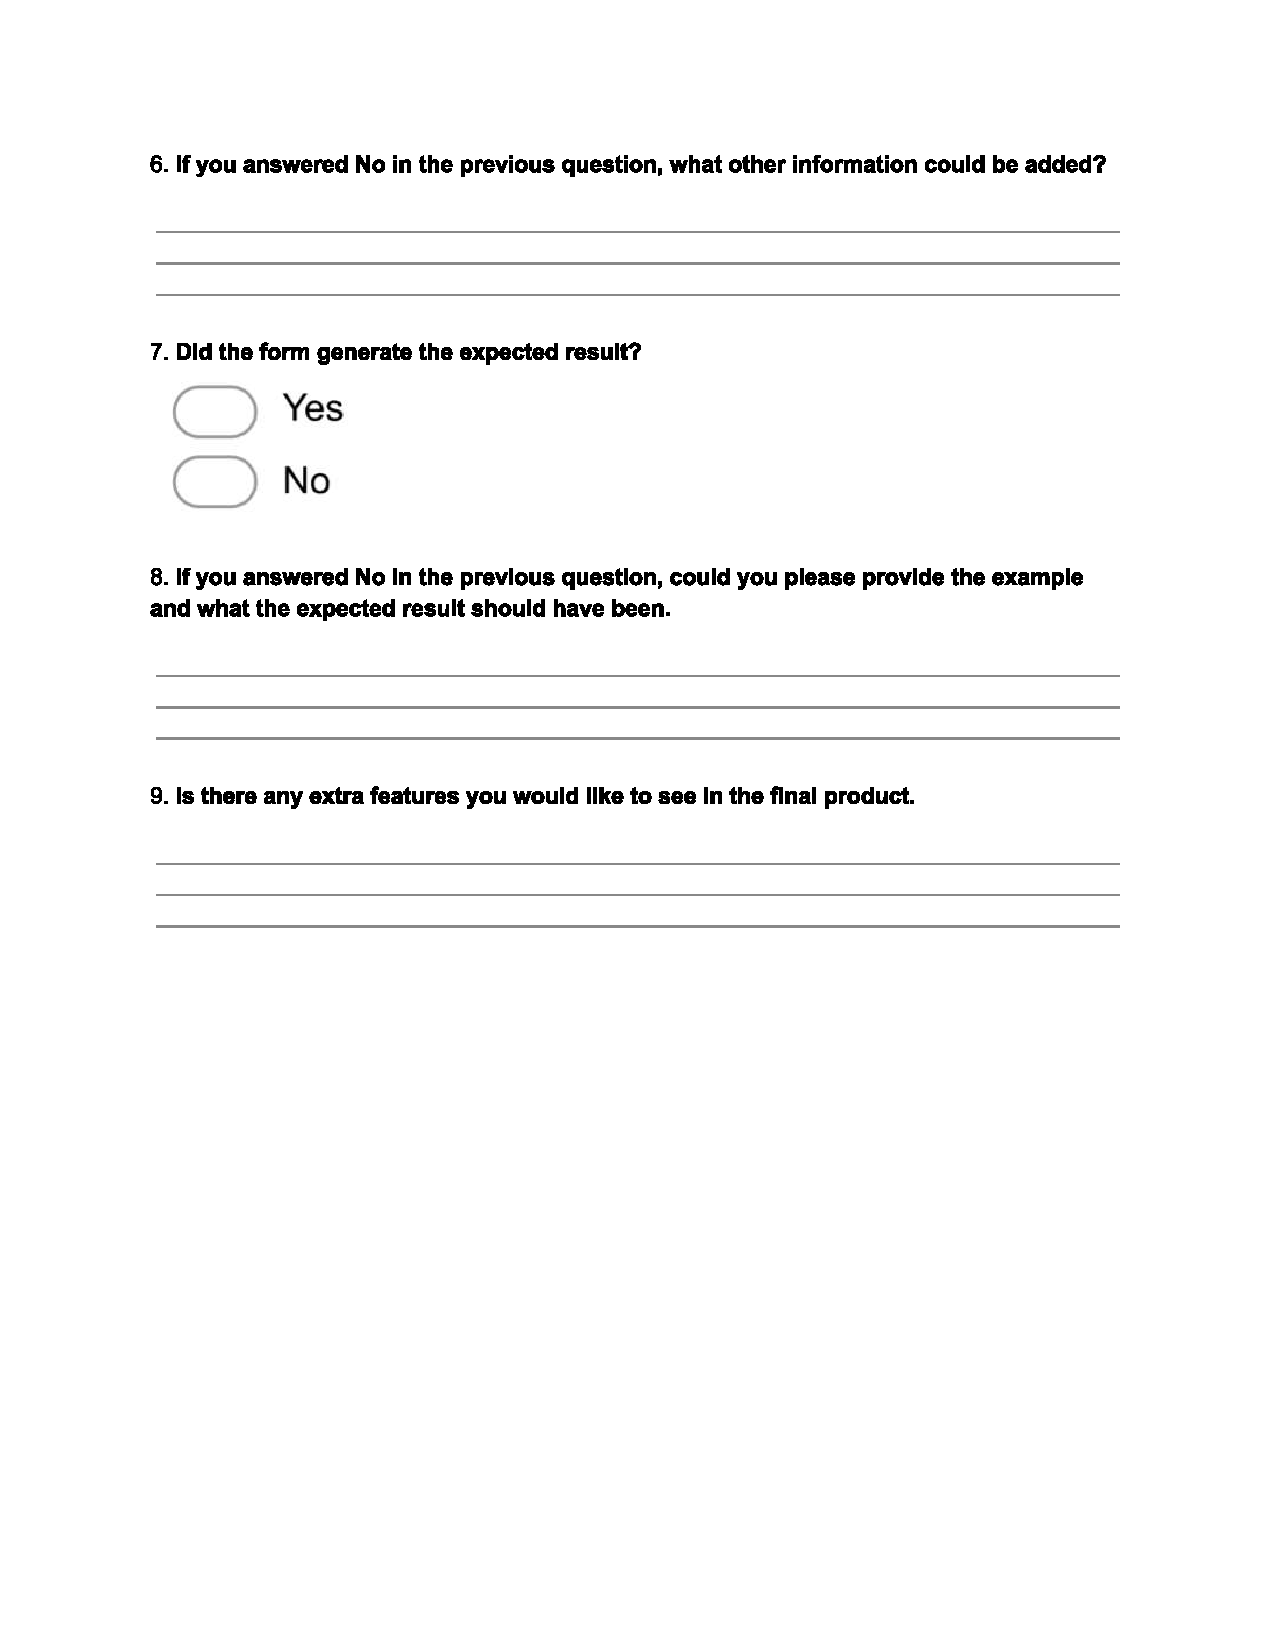
\includegraphics[trim = 40 160 0 60,scale=0.9]{forms/prototypeEvaluationFormPage2.pdf}
\end{centering}

\chapter{Final Usability Study} \label{chp:finalUsabilityStudy}

\newpage
\section{Consent Form}
\vspace{3em}

\begin{centering}
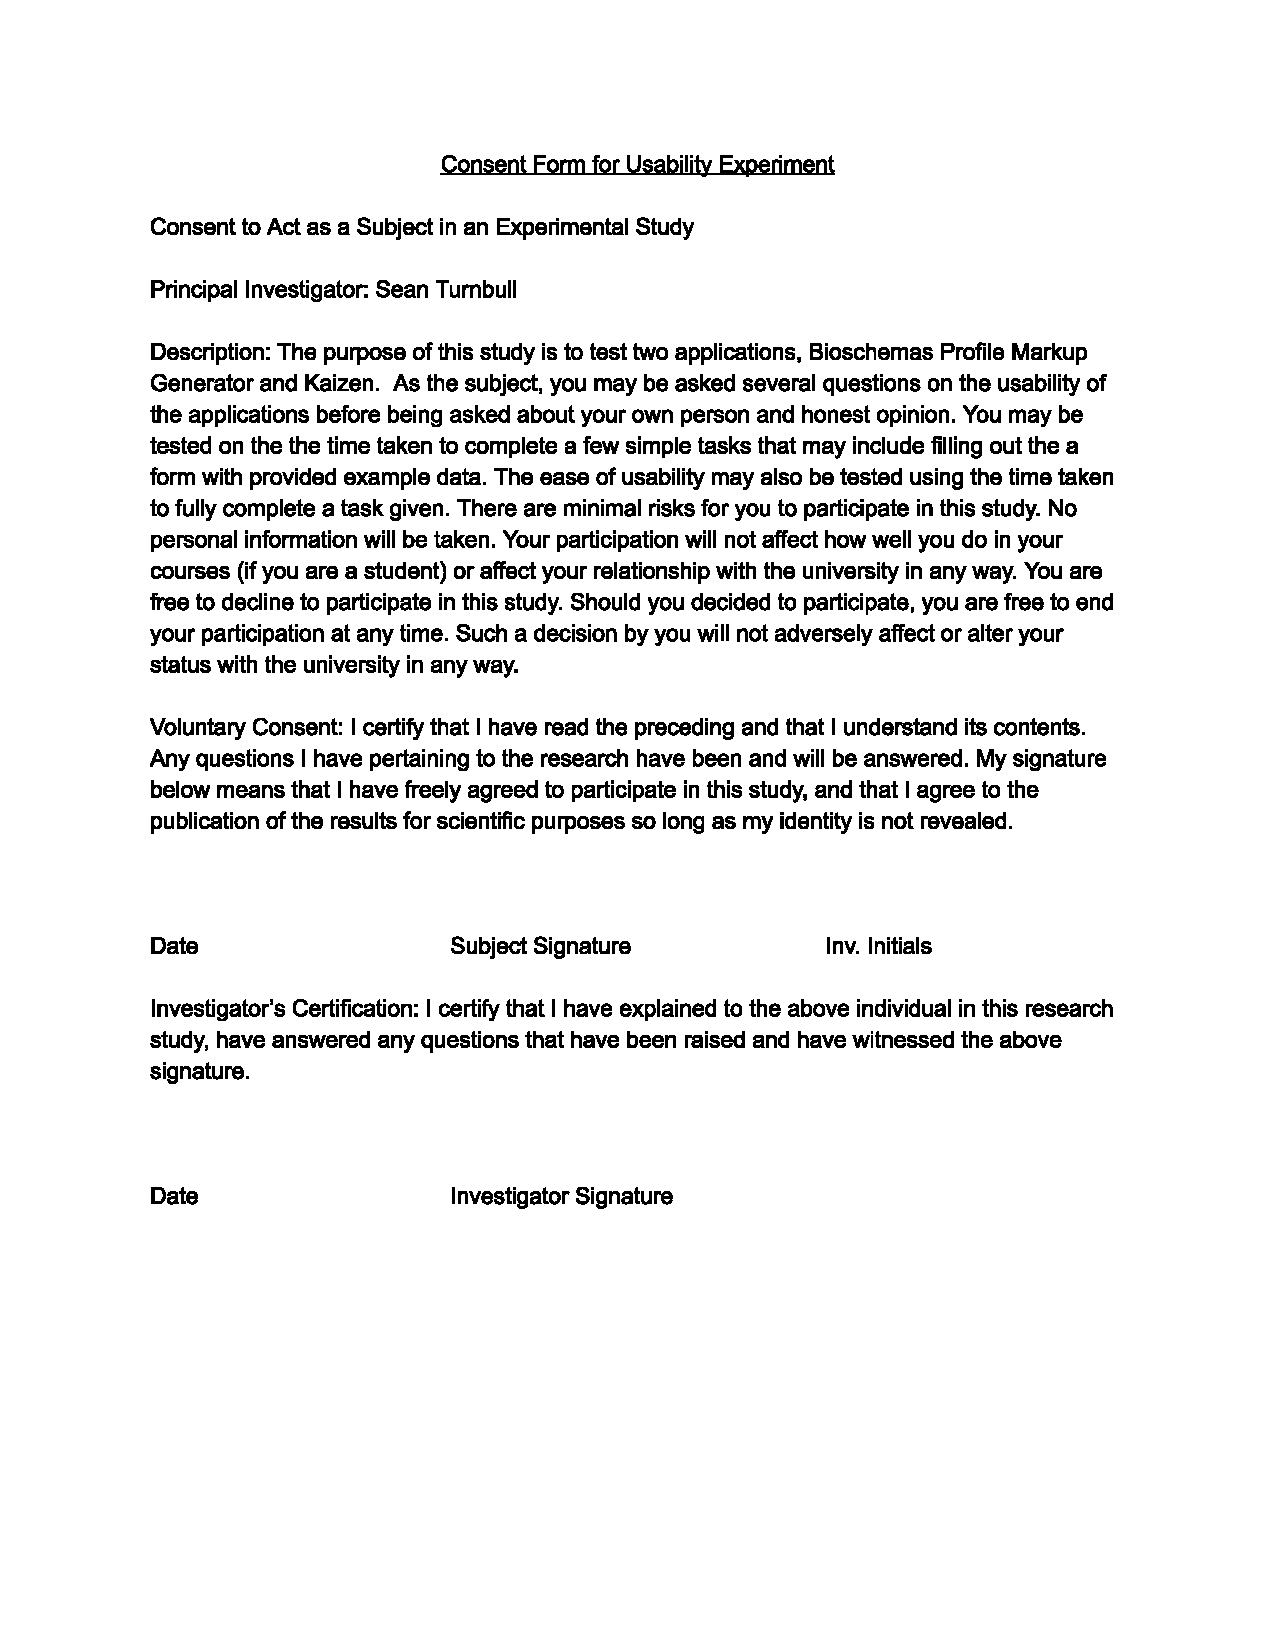
\includegraphics[trim = 40 160 0 60,scale=0.9]{ConsentForm.pdf}
\end{centering}



\newpage
\section{Task Sheets}

\subsection*{System A}
{\setstretch{1.3}
{\color{blue}System A Usability Test}

\noindent
The purpose of this test is to evaluate how easy the developed Bioschemas Profile Markup Generator web application is to use. 

\noindent
You will be timed for each task.

\noindent
Please complete the tasks below.

\noindent
\textbf{Task 1: Generate a markup for the DataCatalog profile. Insert the following data:}

\noindent
Name:\newline
\texttt{OMA Orthology Database}

\noindent
Description:\newline
\texttt{OMA is a project that aims to identify orthologs among publicly available, complete genomes.}

\noindent
Keywords:\newline
\texttt{evolutionary relation, orthology prediction, paralogy}

\noindent
Provider:\newline
\hspace*{35pt}Organization:\newline
\hspace*{70pt}URL: \url{https://www.sib.swiss/}

\noindent
\textbf{Task 2: Download the result from Task 1 into a HTML File.}

\noindent
\textbf{Task 3: Find the Controlled Vocabulary for the Recommended property “encodes” in the Gene Profile.}

\noindent
\textbf{Task 4: Generate a markup for the Gene profile. Insert the following data:}


\noindent
Identifier:\newline
\hspace*{35pt}Property Value:\newline
\hspace*{70pt}URL: \url{http://identifiers.org/ensembl:ENSG00000142192}

\noindent
Name:\newline
\texttt{APP}

\noindent
Encodes:\newline
\hspace*{35pt}BioChemEntity:\newline
\hspace*{70pt}Name: \texttt{Protein P05067}\newline
\hspace*{70pt}Identifier: \texttt{uniprotkb:P05067}\newline
\hspace*{70pt}URL: \url{http://identifiers.org/ensembl:ENSG00000142192}

}


\newpage
\subsection*{System B}

{\setstretch{1.3}
{\color{blue}System B Usability Test}

\noindent
The purpose of this test is to evaluate how easy the developed Kaizen web application is to use. 

\noindent
You will be timed for each task.

\noindent
Please complete the tasks below.

\noindent
\textbf{Task 1: Generate a markup for the DataCatalog profile. Insert the following data:}

\noindent
Name:\newline
\texttt{OMA Orthology Database}

\noindent
Description:\newline
\texttt{OMA is a project that aims to identify orthologs among publicly available, complete genomes.}

\noindent
Keywords:\newline
\texttt{evolutionary relation, orthology prediction, paralogy}

\noindent
Provider:\newline
\hspace*{35pt}Organization:\newline
\hspace*{70pt}URL: \url{https://www.sib.swiss/}

\noindent
\textbf{Task 2: Download the result from Task 1 into a HTML File.}

\noindent
\textbf{Task 3: Find the Controlled Vocabulary for the Recommended property “encodes” in the Gene Profile.}
}

\newpage
\section{Questionnaire}
\vspace*{3.7em}
\begin{centering}

\includegraphics[trim = 40 160 0 60,scale=0.9]{forms/finalEvaluationPage1.pdf}
\end{centering}

\newpage
\begin{centering}

\includegraphics[trim = 40 160 0 60,scale=0.9]{forms/finalEvaluationPage2.pdf}
\end{centering}

\newpage
\section{Task Times}

\subsection*{Task 1}
\begin{figure}[!h]
  \centering
  \begin{minipage}[b]{0.47\textwidth}
    \fbox{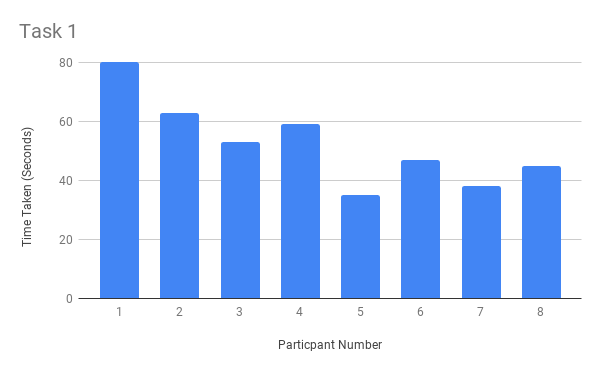
\includegraphics[width=\textwidth]{charts/Tasks/Task_1_System_A.png}}
    \caption{Final Evaluation Task 1: System A}
  \end{minipage}
  \hfill
  \begin{minipage}[b]{0.47\textwidth}
    \fbox{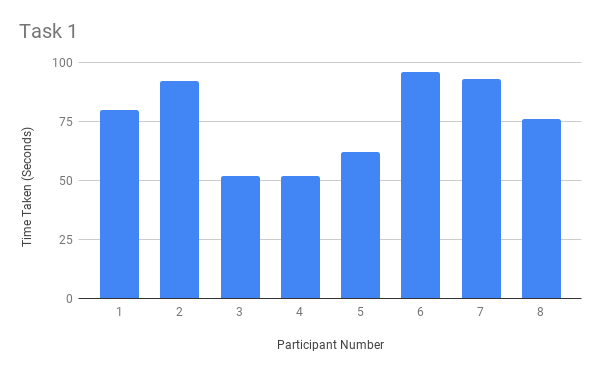
\includegraphics[width=\textwidth]{charts/Tasks/Task_1_System_B.png}}
  \caption{Final Evaluation Task 1: System B}
  \end{minipage}
\end{figure}

\subsection*{Task 2}
\begin{figure}[!h]
  \centering
  \begin{minipage}[b]{0.47\textwidth}
    \fbox{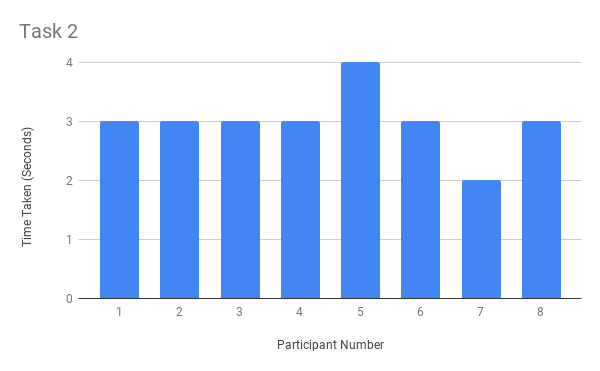
\includegraphics[width=\textwidth]{charts/Tasks/Task_2_System_A.png}}
    \caption{Final Evaluation Task 2: System A}
  \end{minipage}
  \hfill
  \begin{minipage}[b]{0.47\textwidth}
    \fbox{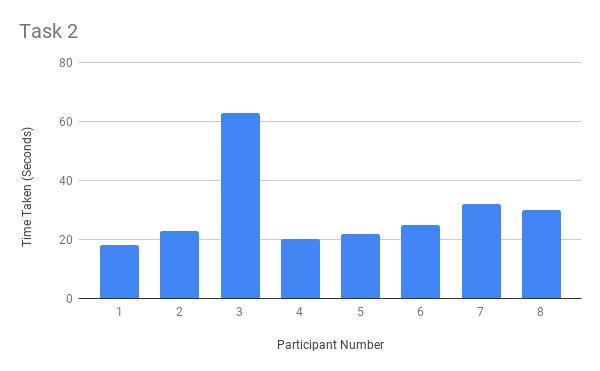
\includegraphics[width=\textwidth]{charts/Tasks/Task_2_System_B.png}}
  \caption{Final Evaluation Task 2: System B}
  \end{minipage}
\end{figure}

\newpage
\subsection*{Task 3}
\begin{figure}[!h]
  \centering
  \begin{minipage}[b]{0.47\textwidth}
    \fbox{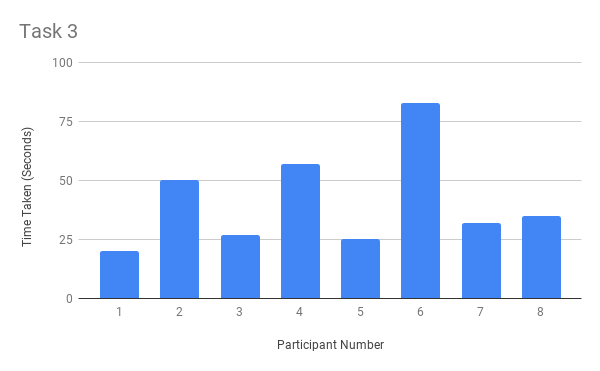
\includegraphics[width=\textwidth]{charts/Tasks/Task_3_System_A.png}}
    \caption{Final Evaluation Task 3: System A}
  \end{minipage}
  \hfill
  \begin{minipage}[b]{0.47\textwidth}
    \fbox{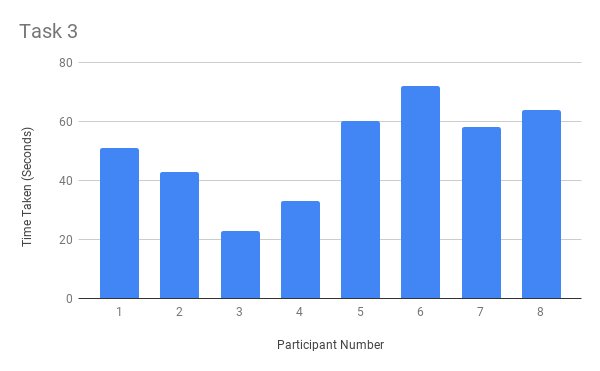
\includegraphics[width=\textwidth]{charts/Tasks/Task_3_System_B.png}}
  \caption{Final Evaluation Task 3: System B}
  \end{minipage}
\end{figure}

\subsection*{Task 4}
\begin{figure}[!h]
  \centering
  \begin{minipage}[b]{0.47\textwidth}
    \fbox{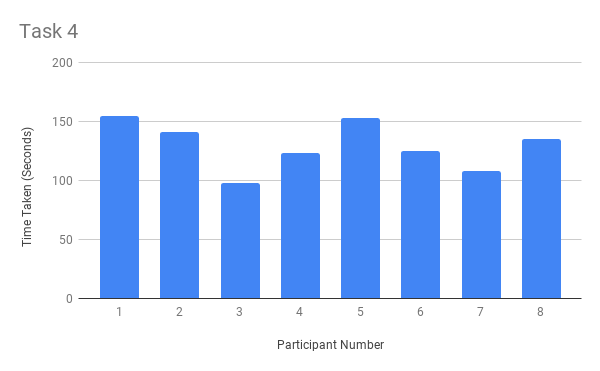
\includegraphics[width=\textwidth]{charts/Tasks/Task_4_System_A.png}}
    \caption{Final Evaluation Task 4: System A}
  \end{minipage}
\end{figure}

\newpage
\subsection*{Task Averages}
\begin{figure}[!h]
  \centering
  \begin{minipage}[b]{0.47\textwidth}
    \fbox{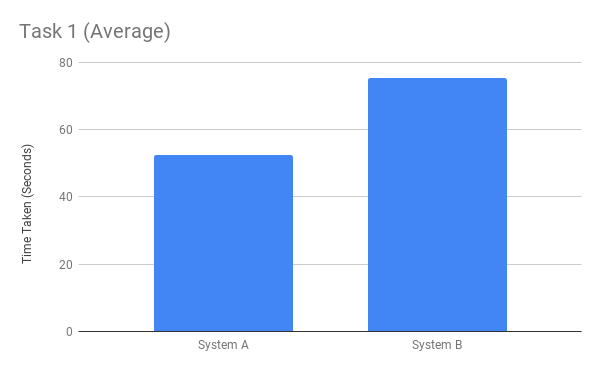
\includegraphics[width=\textwidth]{charts/Tasks/Task_1_(Average).png}}
    \caption{Final Evaluation Task 1: Average}
  \end{minipage}
  \hfill
  \begin{minipage}[b]{0.47\textwidth}
    \fbox{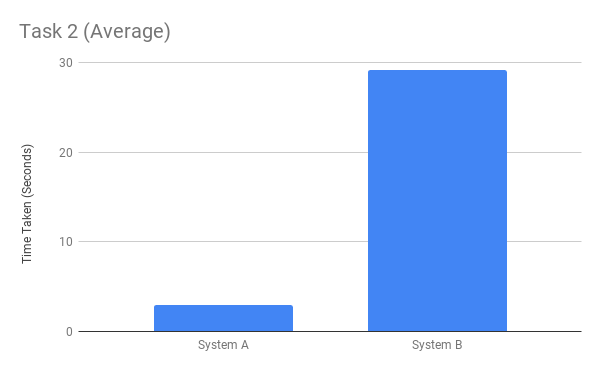
\includegraphics[width=\textwidth]{charts/Tasks/Task_2_(Average).png}}
  \caption{Final Evaluation Task 2: Average}
  \end{minipage}
\end{figure}
\begin{figure}[!h]
  \centering
  \begin{minipage}[b]{0.47\textwidth}
    \fbox{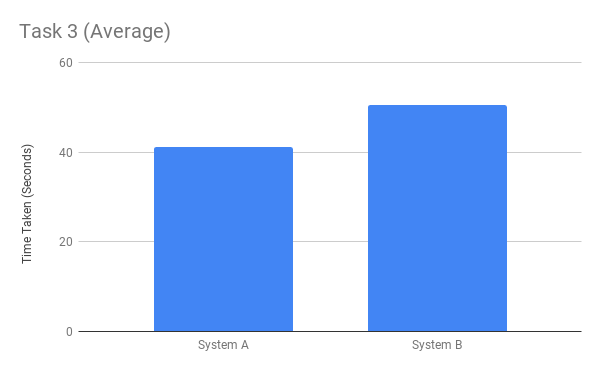
\includegraphics[width=\textwidth]{charts/Tasks/Task_3_(Average).png}}
    \caption{Final Evaluation Task 3: Average}
  \end{minipage}
  \hfill
  \begin{minipage}[b]{0.47\textwidth}
    \fbox{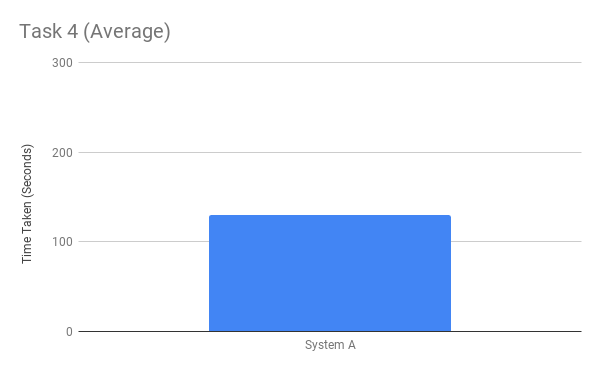
\includegraphics[width=\textwidth]{charts/Tasks/Task_4_(Average).png}}
  \caption{Final Evaluation Task 4: Average}
  \end{minipage}
\end{figure}